\documentclass[12pt]{article}

\author{Matthew D. Cocci}
\title{Asset Pricing}
\date{\today}

%% Formatting & Spacing %%%%%%%%%%%%%%%%%%%%%%%%%%%%%%%%%%%%

%\usepackage[top=1in, bottom=1in, left=1in, right=1in]{geometry} % most detailed page formatting control
\usepackage{fullpage} % Simpler than using the geometry package; std effect
\usepackage{setspace}
%\onehalfspacing
\usepackage{microtype}

%% Formatting %%%%%%%%%%%%%%%%%%%%%%%%%%%%%%%%%%%%%%%%%%%%%

%\usepackage[margin=1in]{geometry}
    %   Adjust the margins with geometry package
%\usepackage{pdflscape}
    %   Allows landscape pages
%\usepackage{layout}
    %   Allows plotting of picture of formatting
\usepackage{multicol}
\setlength{\columnsep}{1cm}



%% Header %%%%%%%%%%%%%%%%%%%%%%%%%%%%%%%%%%%%%%%%%%%%%%%%%

%\usepackage{fancyhdr}
%\pagestyle{fancy}
%\lhead{}
%\rhead{}
%\chead{}
%\setlength{\headheight}{15.2pt}
    %   Make the header bigger to avoid overlap

%\fancyhf{}
    %   Erase header settings

%\renewcommand{\headrulewidth}{0.3pt}
    %   Width of the line

%\setlength{\headsep}{0.2in}
    %   Distance from line to text


%% Mathematics Related %%%%%%%%%%%%%%%%%%%%%%%%%%%%%%%%%%%

\usepackage{amsmath}
\usepackage{amssymb}
\usepackage{amsfonts}
\usepackage{mathrsfs}
\usepackage{amsthm} %allows for labeling of theorems
\theoremstyle{plain}
\newtheorem{thm}{Theorem}[section]
\newtheorem{lem}[thm]{Lemma}
\newtheorem{prop}[thm]{Proposition}
\newtheorem{cor}[thm]{Corollary}
\newtheorem{ax}[thm]{Axiom}

\theoremstyle{definition}
\newtheorem{defn}[thm]{Definition}
\newtheorem{ex}[thm]{Example}
\newtheorem{assump}[thm]{Assumption}

\theoremstyle{remark}
\newtheorem*{rmk}{Remark}
\newtheorem*{note}{Note}

% Below supports left-right alignment in matrices so the negative
% signs don't look bad
\makeatletter
\renewcommand*\env@matrix[1][c]{\hskip -\arraycolsep
  \let\@ifnextchar\new@ifnextchar
  \array{*\c@MaxMatrixCols #1}}
\makeatother


%% Font Choices %%%%%%%%%%%%%%%%%%%%%%%%%%%%%%%%%%%%%%%%%

\usepackage[T1]{fontenc}
\usepackage{lmodern}
\usepackage[utf8]{inputenc}
%\usepackage{blindtext}
\usepackage{courier}


%% Figures %%%%%%%%%%%%%%%%%%%%%%%%%%%%%%%%%%%%%%%%%%%%%%

\usepackage{tikz}
%\usepackage{tikz-3dplot}
\usetikzlibrary{decorations.pathreplacing}
\usetikzlibrary{patterns}
\usepackage{graphicx}
\usepackage{subfigure}
    %   For plotting multiple figures at once
%\graphicspath{ {Directory/} }
    %   Set a directory for where to look for figures

%\pgfdeclarepatternformonly[\LineSpace]{my north east lines}{\pgfqpoint{-1pt}{-1pt}}{\pgfqpoint{\LineSpace}{\LineSpace}}{\pgfqpoint{\LineSpace}{\LineSpace}}%
%{
    %\pgfsetlinewidth{0.4pt}
    %\pgfpathmoveto{\pgfqpoint{0pt}{0pt}}
    %\pgfpathlineto{\pgfqpoint{\LineSpace + 0.1pt}{\LineSpace + 0.1pt}}
    %\pgfusepath{stroke}
%}

%\pgfdeclarepatternformonly[\LineSpace]{my north west lines}{\pgfqpoint{-1pt}{-1pt}}{\pgfqpoint{\LineSpace}{\LineSpace}}{\pgfqpoint{\LineSpace}{\LineSpace}}%
%{
    %\pgfsetlinewidth{0.4pt}
    %\pgfpathmoveto{\pgfqpoint{0pt}{\LineSpace}}
    %\pgfpathlineto{\pgfqpoint{\LineSpace + 0.1pt}{-0.1pt}}
    %\pgfusepath{stroke}
%}

%\newdimen\LineSpace
%\tikzset{
    %line space/.code={\LineSpace=#1},
    %line space=3pt
%}


%% Hyperlinks %%%%%%%%%%%%%%%%%%%%%%%%%%%%%%%%%%%%%%%%%%%%
\usepackage{hyperref}
\hypersetup{%
    colorlinks,
        %   This colors the links themselves, not boxes
    citecolor=black,
        %   Everything here and below changes link colors
    filecolor=black,
    linkcolor=black,
    urlcolor=black
}

%% Colors %%%%%%%%%%%%%%%%%%%%%%%%%%%%%%%%%%%%%%%%%%%%%%%

\usepackage{color}
\definecolor{codegreen}{RGB}{28,172,0}
\definecolor{codelilas}{RGB}{170,55,241}

% David4 color scheme
\definecolor{d4blue}{RGB}{100,191,255}
\definecolor{d4gray}{RGB}{175,175,175}
\definecolor{d4black}{RGB}{85,85,85}
\definecolor{d4orange}{RGB}{255,150,100}


%% Including Code %%%%%%%%%%%%%%%%%%%%%%%%%%%%%%%%%%%%%%%

\usepackage{verbatim}
    %   For including verbatim code from files, no colors
\usepackage{listings}
    %   For including code snippets written directly in this doc

\lstdefinestyle{bash}{%
  language=bash,%
  basicstyle=\footnotesize\ttfamily,%
  showstringspaces=false,%
  commentstyle=\color{gray},%
  keywordstyle=\color{blue},%
  xleftmargin=0.25in,%
  xrightmargin=0.25in
}

\lstdefinestyle{matlab}{%
  language=Matlab,%
  basicstyle=\footnotesize\ttfamily,%
  breaklines=true,%
  morekeywords={matlab2tikz},%
  keywordstyle=\color{blue},%
  morekeywords=[2]{1}, keywordstyle=[2]{\color{black}},%
  identifierstyle=\color{black},%
  stringstyle=\color{codelilas},%
  commentstyle=\color{codegreen},%
  showstringspaces=false,%
    %   Without this there will be a symbol in
    %   the places where there is a space
  numbers=left,%
  numberstyle={\tiny \color{black}},%
    %   Size of the numbers
  numbersep=9pt,%
    %   Defines how far the numbers are from the text
  emph=[1]{for,end,break,switch,case},emphstyle=[1]\color{red},%
    %   Some words to emphasise
}

\newcommand{\matlabcode}[1]{%
    \lstset{style=matlab}%
    \lstinputlisting{#1}
}
    %   For including Matlab code from .m file with colors,
    %   line numbering, etc.

%% Bibliographies %%%%%%%%%%%%%%%%%%%%%%%%%%%%%%%%%%%%

\usepackage{natbib}
    %---For bibliographies
%\setlength{\bibsep}{3pt} % Set how far apart bibentries are


%% Misc %%%%%%%%%%%%%%%%%%%%%%%%%%%%%%%%%%%%%%%%%%%%%%

\usepackage{enumitem}
    %   Has to do with enumeration
\usepackage{appendix}
%\usepackage{natbib}
    %   For bibliographies
\usepackage{pdfpages}
    %   For including whole pdf pages as a page in doc


%% User Defined %%%%%%%%%%%%%%%%%%%%%%%%%%%%%%%%%%%%%%%%%%

%\newcommand{\nameofcmd}{Text to display}
\newcommand*{\Chi}{\mbox{\large$\chi$}} %big chi
    %   Bigger Chi

% In math mode, Use this instead of \munderbar, since that changes the
% font from math to regular
\makeatletter
\def\munderbar#1{\underline{\sbox\tw@{$#1$}\dp\tw@\z@\box\tw@}}
\makeatother

% Misc Math
\newcommand{\ra}{\rightarrow}
\newcommand{\diag}{\text{diag}}
\newcommand{\proj}{\operatorname{proj}}
\newcommand{\ch}{\text{ch}}
\newcommand{\dom}{\text{dom}}
\newcommand{\one}[1]{\mathbf{1}_{#1}}


% Command to generate new math commands:
% - Suppose you want to refer to \boldsymbol{x} as just \bsx, where 'x'
%   is any letter. This commands lets you generate \bsa, \bsb, etc.
%   without copy pasting \newcommand{\bsa}{\boldsymbol{a}} for each
%   letter individually. Instead, just include
%
%     \generate{bs}{\boldsymbol}{a,...,z}
%
% - Uses pgffor package to loop
% - Example with optional argument. Will generate \bshatx to represent
%   \boldsymbol{\hat{x}} for all letters x
%
%     \generate[\hat]{bshat}{\boldsymbol}{a,...,z}

\newcommand{\generate}[4][]{%
  % Takes 3 arguments (maybe four):
  % - 1   wrapcmd (optional, defaults to nothing)
  % - 2   newname
  % - 3   mathmacro
  % - 4   Names to loop over
  %
  % Will produce
  %
  %   \newcommand{\newnameX}{mathmacro{wrapcmd{X}}}
  %
  % for each X in argument 4

  \foreach \x in {#4}{%
    \expandafter\xdef\csname%
      #2\x%
    \endcsname%
    {\noexpand\ensuremath{\noexpand#3{\noexpand#1{\x}}}}
  }
}

% MATHSCR: Gen \sX to stand for \mathscr{X} for all upper case letters
\generate{s}{\mathscr}{A,...,Z}


% BOLDSYMBOL: Generate \bsX to stand for \boldsymbol{X}, all upper and
% lower case.
%
% Letters and greek letters
\generate{bs}{\boldsymbol}{a,...,z}
\generate{bs}{\boldsymbol}{A,...,Z}
\newcommand{\bseta}{\boldsymbol{\eta}}
\newcommand{\bstheta}{\boldsymbol{\theta}}
\newcommand{\bsTheta}{\boldsymbol{\Theta}}
\newcommand{\bsmu}{\boldsymbol{\mu}}
\newcommand{\bsSigma}{\boldsymbol{\Sigma}}
\newcommand{\bssigma}{\boldsymbol{\sigma}}
\newcommand{\bsvarepsilon}{\boldsymbol{\varepsilon}}
\newcommand{\bsalpha}{\boldsymbol{\alpha}}
\newcommand{\bsbeta}{\boldsymbol{\beta}}
\newcommand{\bsgamma}{\boldsymbol{\gamma}}
\newcommand{\bsGamma}{\boldsymbol{\Gamma}}
\newcommand{\bslambda}{\boldsymbol{\lambda}}
\newcommand{\bsLambda}{\boldsymbol{\Lambda}}
\newcommand{\bshatLambda}{\boldsymbol{\hat{\Lambda}}}
\newcommand{\bshatG}{\boldsymbol{\hat{G}}}
\newcommand{\bsdelta}{\boldsymbol{\delta}}
\newcommand{\bsOmega}{\boldsymbol{\Omega}}
\newcommand{\bsPsi}{\boldsymbol{\Psi}}
\newcommand{\bspsi}{\boldsymbol{\psi}}
\newcommand{\bsPhi}{\boldsymbol{\Phi}}

% Special cases like \bshatb for \boldsymbol{\hat{b}}
\generate[\hat]{bshat}{\boldsymbol}{a,b,y,x,X,V,S,W,A,B,P}
\newcommand{\bshatbeta}{\boldsymbol{\hat{\beta}}}
\newcommand{\bshatmu}{\boldsymbol{\hat{\mu}}}
\newcommand{\bshattheta}{\boldsymbol{\hat{\theta}}}
\newcommand{\bsbartheta}{\boldsymbol{\bar{\theta}}}
\newcommand{\bshatSigma}{\boldsymbol{\hat{\Sigma}}}
\newcommand{\bstildebeta}{\boldsymbol{\tilde{\beta}}}
\newcommand{\bstildetheta}{\boldsymbol{\tilde{\theta}}}
\newcommand{\bstildePsi}{\boldsymbol{\tilde{\Psi}}}
\newcommand{\bsbarbeta}{\boldsymbol{\overline{\beta}}}
\newcommand{\bshatOmega}{\boldsymbol{\hat{\Omega}}}
\newcommand{\bsbarg}{\boldsymbol{\overline{g}}}
\newcommand{\bstildey}{\boldsymbol{\tilde{y}}}
\newcommand{\bstildeX}{\boldsymbol{\tilde{X}}}
\newcommand{\bstildevarepsilon}{\boldsymbol{\tilde{\varepsilon}}}
\newcommand{\bstildes}{\boldsymbol{\tilde{s}}}
\newcommand{\bstildeT}{\boldsymbol{\tilde{T}}}
\newcommand{\bstildeC}{\boldsymbol{\tilde{C}}}

% Zero vector as \bso
\renewcommand{\bso}{\boldsymbol{0}}

% Transposes of all the boldsymbol shit
\newcommand{\bsbp}{\boldsymbol{b'}}
\newcommand{\bshatbp}{\boldsymbol{\hat{b'}}}
\newcommand{\bsdp}{\boldsymbol{d'}}
\newcommand{\bsgp}{\boldsymbol{g'}}
\newcommand{\bsGp}{\boldsymbol{G'}}
\newcommand{\bshp}{\boldsymbol{h'}}
\newcommand{\bsSp}{\boldsymbol{S'}}
\newcommand{\bsup}{\boldsymbol{u'}}
\newcommand{\bsxp}{\boldsymbol{x'}}
\newcommand{\bsyp}{\boldsymbol{y'}}
\newcommand{\bsthetap}{\boldsymbol{\theta'}}
\newcommand{\bsmup}{\boldsymbol{\mu'}}
\newcommand{\bsSigmap}{\boldsymbol{\Sigma'}}
\newcommand{\bshatmup}{\boldsymbol{\hat{\mu'}}}
\newcommand{\bshatSigmap}{\boldsymbol{\hat{\Sigma'}}}

% MATHCAL: Gen \calX to stand for \mathcal{X}, all upper case
\generate{cal}{\mathcal}{A,...,Z}

% MATHBB: Gen \X to stand for \mathbb{X} for some upper case
\generate{}{\mathbb}{R,Q,C,Z,N,Z,E}
\newcommand{\Rn}{\mathbb{R}^n}
\newcommand{\RN}{\mathbb{R}^N}
\newcommand{\Rk}{\mathbb{R}^k}
\newcommand{\RK}{\mathbb{R}^K}
\newcommand{\RL}{\mathbb{R}^L}
\newcommand{\Rl}{\mathbb{R}^\ell}
\newcommand{\Rm}{\mathbb{R}^m}
\newcommand{\Rnn}{\mathbb{R}^{n\times n}}
\newcommand{\Rmn}{\mathbb{R}^{m\times n}}
\newcommand{\Rnm}{\mathbb{R}^{n\times m}}
\newcommand{\Rkn}{\mathbb{R}^{k\times n}}
\newcommand{\Cn}{\mathbb{C}^n}
\newcommand{\Cnn}{\mathbb{C}^{n\times n}}

% Dot over
\newcommand{\dx}{\dot{x}}
\newcommand{\ddx}{\ddot{x}}
\newcommand{\dy}{\dot{y}}
\newcommand{\ddy}{\ddot{y}}

% First derivatives
\newcommand{\dydx}{\frac{dy}{dx}}
\newcommand{\dfdx}{\frac{df}{dx}}
\newcommand{\dfdy}{\frac{df}{dy}}
\newcommand{\dfdz}{\frac{df}{dz}}

% Second derivatives
\newcommand{\ddyddx}{\frac{d^2y}{dx^2}}
\newcommand{\ddydxdy}{\frac{d^2y}{dx dy}}
\newcommand{\ddydydx}{\frac{d^2y}{dy dx}}
\newcommand{\ddfddx}{\frac{d^2f}{dx^2}}
\newcommand{\ddfddy}{\frac{d^2f}{dy^2}}
\newcommand{\ddfddz}{\frac{d^2f}{dz^2}}
\newcommand{\ddfdxdy}{\frac{d^2f}{dx dy}}
\newcommand{\ddfdydx}{\frac{d^2f}{dy dx}}


% First Partial Derivatives
\newcommand{\pypx}{\frac{\partial y}{\partial x}}
\newcommand{\pfpx}{\frac{\partial f}{\partial x}}
\newcommand{\pfpy}{\frac{\partial f}{\partial y}}
\newcommand{\pfpz}{\frac{\partial f}{\partial z}}

% argmin and argmax
\DeclareMathOperator*{\argmin}{arg\;min}
\DeclareMathOperator*{\argmax}{arg\;max}
\newenvironment{rcases}
  {\left.\begin{aligned}}
  {\end{aligned}\right\rbrace}

% Various probability and statistics commands
\newcommand{\wn}{\sim\operatorname{WN}}
\newcommand{\iid}{\overset{iid}{\sim}}
\newcommand{\vc}{\operatorname{vec}}
\newcommand{\Cov}{\operatorname{Cov}}
\newcommand{\range}{\operatorname{range}}
\newcommand{\Prb}{\operatorname{P}}
\newcommand{\rank}{\operatorname{rank}}
\newcommand{\trace}{\operatorname{trace}}
\newcommand{\Corr}{\operatorname{Corr}}
\newcommand{\Var}{\operatorname{Var}}
\newcommand{\asto}{\xrightarrow{a.s.}}
\newcommand{\pto}{\xrightarrow{p}}
\newcommand{\msto}{\xrightarrow{m.s.}}
\newcommand{\dto}{\xrightarrow{d}}
\newcommand{\Lpto}{\xrightarrow{L_p}}
\newcommand{\Lqto}[1]{\xrightarrow{L_{#1}}}
\newcommand{\plim}{\text{plim}_{n\rightarrow\infty}}

% Redefine real and imaginary from fraktur to plain text
\renewcommand{\Re}{\operatorname{Re}}
\renewcommand{\Im}{\operatorname{Im}}

% Shorter sums: ``Sum from X to Y''
% - sumXY  is equivalent to \sum^Y_{X=1}
% - sumXYz is equivalent to \sum^Y_{X=0}
\newcommand{\sumnN}{\sum^N_{n=1}}
\newcommand{\sumin}{\sum^n_{i=1}}
\newcommand{\sumjn}{\sum^n_{j=1}}
\newcommand{\sumim}{\sum^m_{i=1}}
\newcommand{\sumik}{\sum^k_{i=1}}
\newcommand{\sumiN}{\sum^N_{i=1}}
\newcommand{\sumkn}{\sum^n_{k=1}}
\newcommand{\sumtT}{\sum^T_{t=1}}
\newcommand{\sumninf}{\sum^\infty_{n=1}}
\newcommand{\sumtinf}{\sum^\infty_{t=1}}
\newcommand{\sumnNz}{\sum^N_{n=0}}
\newcommand{\suminz}{\sum^n_{i=0}}
\newcommand{\sumknz}{\sum^n_{k=0}}
\newcommand{\sumtTz}{\sum^T_{t=0}}
\newcommand{\sumninfz}{\sum^\infty_{n=0}}
\newcommand{\sumtinfz}{\sum^\infty_{t=0}}

\newcommand{\prodnN}{\prod^N_{n=1}}
\newcommand{\prodin}{\prod^n_{i=1}}
\newcommand{\prodiN}{\prod^N_{i=1}}
\newcommand{\prodkn}{\prod^n_{k=1}}
\newcommand{\prodtT}{\prod^T_{t=1}}
\newcommand{\prodnNz}{\prod^N_{n=0}}
\newcommand{\prodinz}{\prod^n_{i=0}}
\newcommand{\prodknz}{\prod^n_{k=0}}
\newcommand{\prodtTz}{\prod^T_{t=0}}

% Bounds
\newcommand{\atob}{_a^b}
\newcommand{\ztoinf}{_0^\infty}
\newcommand{\kinf}{_{k=1}^\infty}
\newcommand{\ninf}{_{n=1}^\infty}
\newcommand{\minf}{_{m=1}^\infty}
\newcommand{\tinf}{_{t=1}^\infty}
\newcommand{\nN}{_{n=1}^N}
\newcommand{\tT}{_{t=1}^T}
\newcommand{\kinfz}{_{k=0}^\infty}
\newcommand{\ninfz}{_{n=0}^\infty}
\newcommand{\minfz}{_{m=0}^\infty}
\newcommand{\tinfz}{_{t=0}^\infty}
\newcommand{\tTz}{_{t=0}^T}

% Limits
\newcommand{\limN}{\lim_{N\rightarrow\infty}}
\newcommand{\limn}{\lim_{n\rightarrow\infty}}
\newcommand{\limk}{\lim_{k\rightarrow\infty}}
\newcommand{\limt}{\lim_{t\rightarrow\infty}}
\newcommand{\limT}{\lim_{T\rightarrow\infty}}
\newcommand{\limhz}{\lim_{h\rightarrow 0}}

% Shorter integrals: ``Integral from X to Y''
% - intXY is equivalent to \int^Y_X
\newcommand{\intab}{\int_a^b}
\newcommand{\intzN}{\int_0^N}



%%%%%%%%%%%%%%%%%%%%%%%%%%%%%%%%%%%%%%%%%%%%%%%%%%%%%%%%%%%%%%%%%%%%%%%%
%% BODY %%%%%%%%%%%%%%%%%%%%%%%%%%%%%%%%%%%%%%%%%%%%%%%%%%%%%%%%%%%%%%%%
%%%%%%%%%%%%%%%%%%%%%%%%%%%%%%%%%%%%%%%%%%%%%%%%%%%%%%%%%%%%%%%%%%%%%%%%



\begin{document}
\maketitle

\tableofcontents


\clearpage
\begin{multicols*}{2}
\section{Key Formulas}

\subsection{Prices and Payoffs}

Agent problem: two periods, endowments $e_t$ and $e_{t+1}$, rate
of \emph{time} (but \emph{not} risk) discounting $\beta$. Can buy/sell
any amount of asset,\footnote{
  Critical assumption.
  Implies agent can make \emph{arbitrarily small} portfolio adjustments,
  hence justified in using FOCs to characterize optimum.
  Thus price $p_t$ will be a \emph{marginal} concept---what an investor
  would pay to hold a tiny extra piece of the asset.
  Doesn't work for large venture cap all-or-nothing type investments.
}
price $p_t$, payoff $x_{t+1}$ (RV realized $t+1$).
\begin{align*}
  \max_{\xi\in\R}
  \;
  &u(c_t) + \beta\E_t[u(c_{t+1})] \\
  \text{s.t.}\qquad
  c_t &= e_t - \xi p_t \\
  c_{t+1} &= e_{t+1} + \xi x_{t+1}
\end{align*}
FOCs give price in terms of \emph{stochastic discount factor}
$m_{t+1}$ (also a RV),\footnote{%
  $m_{t+1}$ also sometimes called marginal rate of substitution, state
  price density, change of measure
}
\begin{align}
  p_t = \E_t[m_{t+1}x_{t+1}],
  \quad
  m_t := \beta \frac{u'(c_{t+1})}{u'(c_t)}
  \label{pemx}
  %\\
  %\text{where}\quad
  %m_t :=&\; \beta \frac{u'(c_{t+1})}{u'(c_t)}
  %\label{mdf}
\end{align}
Eq.~\ref{pemx} holds \emph{after} agent has made all
desired investments \& reached optimal allocation.
\footnote{%
  For utility, we often use \emph{power utility}
  $u(c) = \frac{c^{1-\gamma}-1}{1-\gamma}$
  which implies $u(c)=\log(c)$ as $\gamma\ra 1$ and
  $u'(c) = c^{-\gamma}$
}

\emph{Returns} have unit price, RV payoff $R_{t+1}$:
\begin{align}
  1 &= \E_t[m_{t+1}R_{t+1}]
  \label{ret}
\end{align}
Eq.~\ref{pemx} is a map/operator $p[x]$ from RV payoff $x(\omega)$ to
price $p$. Eq.~\ref{ret} is instead a condition that a unit-price asset
(a return) must satisfy.
Payoffs across states $R(\omega)$ co-move with $m(\omega)$
such that Eq.~\ref{ret} holds.

\emph{Excess return} $R^e=R^i-R^j$ is long return $R^i$, short $R^j$.
With both $R^i,R^j$ unit price, portfolio is zero cost:
\begin{align*}
  0 = \E_t[m_{t+1}R^e_{t+1}]
  %= \E_t[m_{t+1}(R^i_{t+1}-R_{t+1}^j)]
\end{align*}
\emph{Risk-free rate} $R^f$ satisfies $\E_t[R^f_{t+1}]=R^f_{t+1}$
(though $R^f_t\neq R^f_s$), hence Eq.~\ref{ret} gives
\begin{align}
  R^f
  &= 1/\;\E[m]
  \label{rf}
\end{align}
To interpret pricing Eq.~\ref{pemx}, use Eq.~\ref{rf} and
$\Cov(x,y)=\E[xy] - \E[x]\E[y]$ on $\E[mx]$:
\begin{align}
  p =  \frac{\E[x]}{R^f} + \Cov(m,x)
  \label{riskadj}
\end{align}
Price is discounted expected payoff plus a risk
correction for covariance of payoff $x$ with $m$.
Risk neutrality implies $u'$, hence $m$, constant, in which case
$\Cov(m,x)=0$.

If $x_{t+1}$ is a return $R^i$, the above becomes
\begin{align}
  \E[R^i] - R^f =  -R^f \Cov(m,R^i)
  \label{riskadjret}
\end{align}
Thus assets only generate average excess (above $R^f$) returns if
correlated with $m$.

\subsection{Contingent Claims}

Let $pc(\omega)$ denote price of a \emph{contingent claim} paying \$1
if state $\omega$ realized, \$0 otherwise.
Assume \emph{complete markets} with a contingent claim traded
for each $\omega$, hence $pc(\omega)$ defined $\forall
\omega\in\Omega$.\footnote{
  Don't strictly need contingent claims $\forall\omega$.
  But must be able to synthesize/replicate with other traded assets.
  If fewer assets traded than total no. of states, can get
  complete markets if \emph{dynamic trading} allowed.
}
Can price any payoff $x:\Omega\ra\R$
\begin{align}
  p[x]
  = \sum_\omega pc(\omega) x(\omega)
  \label{eq:contingentprice}
\end{align}
Letting $\pi(\omega)$ denote state probs, can get discount factor $m$
and pricing Eq.~\ref{pemx}
\begin{align*}
  p[x]
  &= \sum_\omega
  \pi(\omega)
  \underbrace{%
  \left(
  \frac{pc(\omega)}{\pi(\omega)}
  \right)
  }_{m(\omega)}
  x(\omega)
  = \E[mx]
\end{align*}
Alternatively, can also rewrite Equation~\ref{eq:contingentprice} using
\emph{risk neutral probs} $\pi^*(\omega)$
\begin{align*}
  p[x]
  &= \frac{1}{R^f} \sum_\omega
  \underbrace{R^f pc(\omega)}_{\pi^*(\omega)}x(\omega)
  = \frac{\E^*[x(\omega)]}{R^f}
\end{align*}


\clearpage
\subsection{Continuous Time}

Agent maximizes utility given endowment by buying/selling asset over
time, which pays dividends continuously at rate $D_t$ per unit time and
has price $p_t$ following a diffusion:\footnote{%
  Price follows
  $dp_t/p_t = \mu(\,\cdot\,)\; dt + \sigma(\,\cdot\,) \; dW_t$
  where $\mu(\,\cdot\,)$ and $\sigma(\,\cdot\,)$ are functions that can
  depend upon $t$, $p_t$, or other state variables, allowing
  us to generate non-Gaussian dynamics (though $W_t$ normal).
}
\begin{align*}
  \max \;
  \E_t \int_{0}^\infty e^{-\rho s} u(c_{t+s})\; ds
\end{align*}
FOCs involving $\Lambda_t$, analogue of SDF $m_{t+1}$ that represents
discounted level of MU:
%\begin{align*}
  %p_tu'(c_t)
  %= \E_t
  %\int_{0}^\infty e^{-\delta s} u'(c_{t+s})D_{t+s}\; ds
%\end{align*}
%Equivalently, we have
\begin{align}
  p_t\Lambda_t
  =&\; \E_t
  \int_{0}^\infty \Lambda_{t+s}D_{t+s}\; ds
  \label{pemxcont1}
  \\
  \Lambda_t :=&\; e^{-\rho t} u'(c_t)
\end{align}
Difference Eq.~\ref{pemxcont1} between $t+\Delta$ and $t$, take cond.
exp. $\E_t$ of both sides, send $\Delta\ra 0$, rearrange to get
fundamental pricing eq.
%\begin{align*}
  %\E_t
  %\left[
  %\Lambda_{t+\Delta}p_{t+\Delta}
  %-\Lambda_tp_t
  %\right]
  %\\
  %&= \E_t\left[
  %\int_{0}^\infty \Lambda_{t+\Delta+s}D_{t+\Delta+s}\; ds
  %-
  %\int_{0}^\infty \Lambda_{t+s}D_{t+s}\; ds
  %\right]
  %\\
  %&=
  %-\E_t
  %\int_{0}^\Delta \Lambda_{t+s}D_{t+s}\; ds
  %\\
  %\implies\quad
%\end{align*}
%Sending $\Delta\ra 0$ and rearranging, we get
%fundamental pricing equation
\begin{align}
  \boxed{%
  0 = \Lambda_t D_t \;dt + \E_t[d(\Lambda_tp_t)]
  }
  \label{pemxcont2}
\end{align}
If $D_t=0$, martingale MU-weighted price.

Use Ito's Lemma to break up $d(\Lambda_tp_t)$, obtain equivalent
fundamental pricing eqn:
\begin{align*}
  \boxed{%
  0 = \Lambda D \,dt
  + \E_t[p \,d\Lambda + \Lambda \, dp + d\Lambda \,dp]
  }
  %\label{pemxcont3}
\end{align*}
If $\Lambda$ and $p$ never zero, divide through by $\Lambda p$:
\begin{align}
  \boxed{%
  0 = \frac{D}{p} \,dt
  + \E_t\left[
    \frac{d\Lambda}{\Lambda} + \frac{dp}{p}
    + \frac{d\Lambda}{\Lambda}\frac{dp}{p}
    \right]
  }
  \label{pemxcont4}
\end{align}
Now \emph{returns}.
Holding the asset at $t$ earns total \emph{net payoff} $dp_t + D_t dt$
over the next instant. Hence total instantaneous \emph{net return} at
$t$
%(denoted $dR_t$\footnote{
  %To see that $dR_t$ is the proper notation for a net return, consider a
  %net return in discrete time, which equals
  %$R_{t+1}-1= (p_{t+1}+D_{t+1})/p_t - p_t/p_t=R_{t+1}-R_t$.
%})
is given by that net payoff over price
\begin{align}
  %dR_t =
  \frac{dp_t}{p_t}
  + \frac{D_t}{p_t} dt
  \label{returnscont}
\end{align}
The \emph{risk free asset} pays instantaneous net return
%$dR_t=r^f_t dt$,
$r^f_t dt$.\footnote{%
  $r^f_t$ is the level of the risk free rate at $t$.
  As in discrete time, even though $r^f_t\neq r^f_s$ in general, it is
  ``risk free'' in sense that the net rate of return over the next
  instant has no Brownian term and is simply $r^f_t\;dt$.
}
Equating with Eq.~\ref{returnscont}, we see two ways to model this
asset: (i) Constant $p_t=1$ with $D_t=r_t^f$
or (ii) $dp_t/p_t=r^f_t\;dt$ with $D_t=0$.
Using either in Eq.~\ref{pemxcont4}, we can get the continuous time
analog of Eq.~\ref{rf}:
\begin{align}
  r^f_t\;dt =
  -\E_t\left[ \frac{d\Lambda_t}{\Lambda_t} \right]
  \label{rfcts}
\end{align}
Now use Eq.~\ref{rfcts} to get the continuous time analog of the risk
adjustment formula (\ref{riskadjret})
\begin{align*}
  \E_t\left[
     \frac{dp_t}{p_t}
  \right]
  +
  \frac{D_t}{p_t} dt
  =
  r^f_t\;dt
  - \E_t\left[
     \frac{d\Lambda_t}{\Lambda_t}\frac{dp_t}{p_t}
    \right]
  %\label{pemxcont5}
\end{align*}


\clearpage
\subsection{State Space Geometry}

For this section, assume finite state space
$\Omega=\{\omega_1,\ldots,\omega_S\}$.\footnote{%
  Everything generalizes to the infinite case with careful math.
}
Therefore, any state-contingent payoff $x(\omega)$ can be represented as
a vector in $\R^S$
\begin{align*}
  \bsx
  &:= \big(x(\omega_1),\; \ldots,\; x(\omega_S)\big)'
  \in\R^S
\end{align*}
Define \emph{payoff space} $\underline{X}\subseteq \R^S$ as the set of
all payoffs that can be bought, sold, or synthesized
$a\bsx_1 + b\bsx_2$ for $a,b\in\R$ and $\bsx_1,\bsx_2\in\underline{X}$.
(Assumes free portfolio formation, i.e. no bid-ask
spread, short-sale constraints, etc.)

A market is \emph{complete} if $\underline{X}=\R^S$, \emph{incomplete}
if $\underline{X}\subsetneq\R^S$. In a complete market, contingent
claims to all states of nature either exist or can be
replicated/synthesized.

\subsubsection{Complete Markets}

Contingent claim price vector $\underline{X}=\R^S$:
\begin{align*}
  \bsp\bsc
  &:= \big(pc(\omega_1),\; \ldots,\; pc(\omega_S)\big)'
  \in\R^S
\end{align*}
Hence pricing Eq.~\ref{eq:contingentprice} is just an inner product
\begin{align}
  p[x]=\langle \bsp\bsc, \bsx\rangle
  = \lVert \bsp\bsc\rVert \times \lVert \proj(\bsx|\bsp\bsc)\rVert
  \label{vectorprice}
\end{align}
Second equality is a property of inner products. It implies
\emph{identical price hyperplanes} in $\R^{S-1}$, which lie at right
angles to $\bsp\bsc\in\R^S$ \& connect payoffs $\bsx\in\R^S$ of
identical price.
If $S=2$, the payoff space looks like
\vspace{10pt}

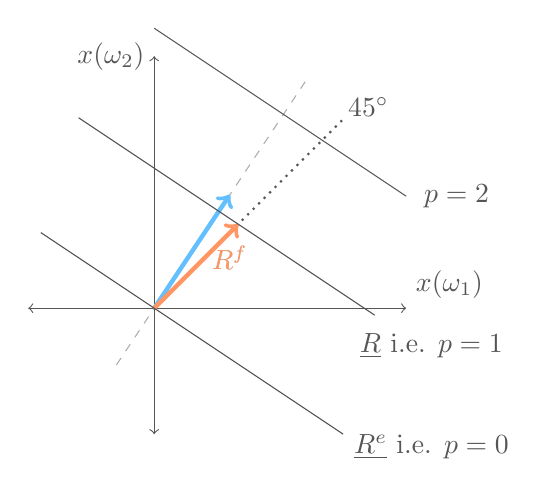
\begin{tikzpicture}[xscale=1.6, yscale=1.6] %, shorten >= 3pt
  % Axes
  \draw[d4black, <->] (0,-1) -- (0,0) -- (0,2)
                      node[left]{$x(\omega_2)$};
  \draw[d4black, <->] (-1,0) -- (0,0) -- (2,0)
                      node[above right]{$x(\omega_1)$};

  % Contingent claims price vector, pc = (0.6, 0.9)
  % Hence p = 0.6x1 + 0.9x2 => x2 = (10/9)p - (2/3) x1
  \draw[d4gray, dashed] (-0.3,-0.45) -- (1.2,1.8);
  \draw[d4blue, ultra thick, ->] (0.0,0.0) -- (0.6,0.9);
  \node[d4gray] at (0.5,1.05) {$\bsp\bsc$};
  \node[d4blue] at (0.5,1.05) {$\bsp\bsc$};

  % Risk free rate
  \draw[d4black, thick, dotted] (0.0,0.0) -- (1.5,1.5);
  \node[d4black] at (1.7,1.6) {$45^{\circ}$};
  \draw[d4orange, ultra thick, ->] (0.0,0.0) -- (0.6666666,0.6666666);
  \node[d4gray] at (0.6,0.4) {$R^f$};
  \node[d4orange] at (0.6,0.4) {$R^f$};

  % Space of excess returns, x2 = -(2/3) x1
  \draw[d4black, thin] (-0.9, 0.6) -- (1.5, -1.0);
  \node[d4black] at (2.2,-1.1) {$\underline{R^e}$ i.e. $p=0$};

  % Space of returns, x2 = (10/9) - (2/3) x1
  \draw[d4black, thin] (-0.6, 1.5111111) -- (1.75,-0.05555555);
  \node[d4black] at (2.2,-0.3) {$\underline{R}$ i.e. $p=1$};

  % Space of p=2, x2 = (10/9)*2 - (2/3) x1
  \draw[d4black, thin] (0.0, 2.2222222) -- (2,0.88888888);
  \node[d4black] at (2.4,0.888888888) {$p=2$};
\end{tikzpicture}
%\begin{align*}
  %pc &= (0.6, \; 0.9)\\
 %p &= 0.6x_1 +  0.9x_2 \\
  %x_2 &= \frac{10}{9}p - \frac{2}{3}x_1
%\end{align*}

We can also use vector geometry to understand $p=\E[mx]$, i.e.\ pricing
with SDF
\begin{align*}
  \bsm=(m(\omega_1),\ldots,m(\omega_S))\in\R^S
\end{align*}
instead of contingent claims prices $pc(\omega)$.
To do so, simply switch the underlying inner product and norm from
Euclidean to $L^2$:
\begin{align*}
  \langle x,y \rangle := \E[xy]
  \qquad
  \lVert x\rVert := \sqrt{\E[x^2]}
\end{align*}
%What's more, we even have a version of Expression~\ref{vectorprice}:
%\begin{align*}
  %\langle x,y \rangle
  %= \lVert y\rVert \times \lVert \proj(x|y)\rVert
%\end{align*}
\emph{However}, important note:
we will continue to draw vectors, visualize projections, and reason in
Euclidean space. We use this visual metapher \emph{even though} every
dot/inner product is really $\E[xy]$ underneath, involving RVs $x,y$
rather than vectors $\bsx,\bsy$.

For example, we update the picture to
\vspace{10pt}

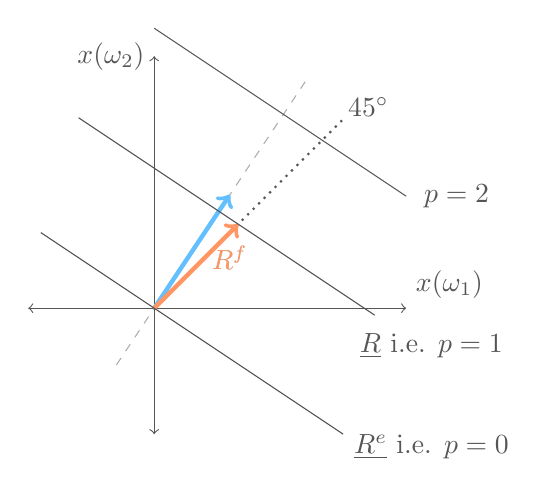
\begin{tikzpicture}[xscale=1.6, yscale=1.6] %, shorten >= 3pt
  % Axes
  \draw[d4black, <->] (0,-1) -- (0,0) -- (0,2)
                      node[left]{$x(\omega_2)$};
  \draw[d4black, <->] (-1,0) -- (0,0) -- (2,0)
                      node[above right]{$x(\omega_1)$};

  % Contingent claims price vector, pc = (0.6, 0.9)
  % Hence p = 0.6x1 + 0.9x2 => x2 = (10/9)p - (2/3) x1
  \draw[d4gray, dashed] (-0.3,-0.45) -- (1.2,1.8);
  \draw[d4blue, ultra thick, ->] (0.0,0.0) -- (0.6,0.9);
  \node[d4gray] at (0.5,1.05) {$\bsp\bsc$};
  \node[d4blue] at (0.5,1.05) {$\bsp\bsc$};

  % Risk free rate
  \draw[d4black, thick, dotted] (0.0,0.0) -- (1.5,1.5);
  \node[d4black] at (1.7,1.6) {$45^{\circ}$};
  \draw[d4orange, ultra thick, ->] (0.0,0.0) -- (0.6666666,0.6666666);
  \node[d4gray] at (0.6,0.4) {$R^f$};
  \node[d4orange] at (0.6,0.4) {$R^f$};

  % Space of excess returns, x2 = -(2/3) x1
  \draw[d4black, thin] (-0.9, 0.6) -- (1.5, -1.0);
  \node[d4black] at (2.2,-1.1) {$\underline{R^e}$ i.e. $p=0$};

  % Space of returns, x2 = (10/9) - (2/3) x1
  \draw[d4black, thin] (-0.6, 1.5111111) -- (1.75,-0.05555555);
  \node[d4black] at (2.2,-0.3) {$\underline{R}$ i.e. $p=1$};

  % Space of p=2, x2 = (10/9)*2 - (2/3) x1
  \draw[d4black, thin] (0.0, 2.2222222) -- (2,0.88888888);
  \node[d4black] at (2.4,0.888888888) {$p=2$};
\end{tikzpicture}

\clearpage
\subsubsection{Incomplete Markets}

Assume $\underline{X}\subsetneq \R^S$, i.e. tradeable assets don't
\emph{span} the state space. For ex, the figure below shows
$\dim(\underline{X})=2<S=3$. $\underline{X}$ is a plane extending out
from the triangle.

\vspace{10pt}
%\tdplotsetmaincoords{70}{15}
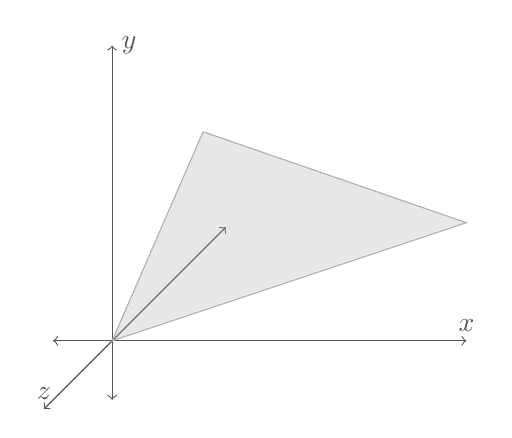
\begin{tikzpicture}[scale=1.5] %,tdplot_main_coords
    % Define axes
    \draw[d4black,<->] (-0.5,0,0) -- (3,0,0) node[above]{$x$};
    \draw[d4black,<->] (0,-0.5,0) -- (0,2.5,0) node[right]{$y$};
    \draw[d4black,<->] (0,0,-2.5) -- (0,0,1.5) node[anchor=south]{$z$};

    % Draw the plane
    \fill[
        draw=d4gray,%
        fill=d4gray,%
        fill opacity=0.3,%
    ] (0,1,-2)
      -- (3,1,0)
      -- (0,0,0)
      -- cycle;

    % Draw reference points
    %\node[d4black] at (0.7,0.7,1.8) {$b$};
\end{tikzpicture}
\\
\emph{Goal}: Suppose we don't have an economic model giving SDF $m$
pricing payoffs $x\in\underline{X}$ according to $p=\E[mx]$.
Can we go backwards and \emph{find} a SDF to price assets?

\begin{assump}
For all $x_1,x_2\in \underline{X}$ and $a,b\in\R$, we might assume
\begin{itemize}
  \item[A1.] \emph{Portfolio formation}:
    $ax_1+bx_2\in\underline{X}$.
  \item[A2.] \emph{Linearity/Law Of One Price} (LOOP):
    $p[ax_1+bx_2] = ap[x_1]+bp[x_2]$.
    \footnote{
      Note: people colloquially use ``no arb'' to refer to
      violations of A2/LOOP, \emph{not} A3 (which is stronger).
    }
  \item[A3.] \emph{No Arbitrage}:
    If $x(\omega)\geq x'(\omega)$ $\forall \omega\in\Omega$,
    strict for at least one $\omega$, $p[x]>p[x']$.

    With A1-2, equivalent to:
    If $x(\omega)\geq 0$ $\forall\omega$,
    strict for at least one, $p[x]>0$.
    (``No free assets that might pay'')
\end{itemize}
\end{assump}

\begin{thm}
We care about two directions
\begin{itemize}
  \item
    \emph{($\Rightarrow$)}
    Given SDF $m$ from an economic model pricing all assets/payoffs in
    $\R^S$ by $p=\E[mx]$, A2 (LOOP) holds.
  \item
    \emph{($\Leftarrow$)}
    Assuming A1 \& A2, $\exists\,!$ a discount factor
    $x^*\in\underline{X}$ pricing all assets in $\underline{X}$,
    i.e. s.t. $p=\E[x^*x]$ for all $x\in\underline{X}$
\end{itemize}
\end{thm}
\begin{proof}
($\Rightarrow$) $p[ax_1+bx_2] = \E[m(ax_1+bx_2)]$. Linearity of
$\E$ to conclude.

($\Leftarrow$) First, A1-2 imply \emph{parallel, linear} price
hyperplanes in $\underline{X}$.
Figure below depicts this for $\dim(\underline{X})=2$.
Dashed line $\perp$ to the price planes
pins down direction of $x^*$.
Then just fix length so $1=\E[x^*R]$ $\forall R\in\underline{R}$.

\vspace{10pt}

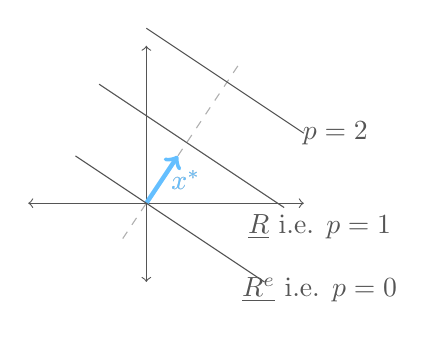
\begin{tikzpicture}[xscale=1, yscale=1] %, shorten >= 3pt
  % Axes
  \draw[d4black, <->] (0,-1) -- (0,0) -- (0,2);
  \draw[d4black, <->] (-1.5,0) -- (0,0) -- (2,0);

  % Contingent claims price vector, pc = (0.6, 0.9)
  % Hence p = 0.6x1 + 0.9x2 => x2 = (10/9)p - (2/3) x1
  \draw[d4gray, dashed] (-0.3,-0.45) -- (1.2,1.8);
  \draw[d4blue, ultra thick, ->] (0.0,0.0) -- (0.4,0.6);
  \node[d4gray] at (0.5,0.3) {$x^*$};
  \node[d4blue] at (0.5,0.3) {$x^*$};

  % Space of excess returns, x2 = -(2/3) x1
  \draw[d4black, thin] (-0.9, 0.6) -- (1.5, -1.0);
  \node[d4black] at (2.2,-1.1) {$\underline{R^e}$ i.e. $p=0$};

  % Space of returns, x2 = (10/9) - (2/3) x1
  \draw[d4black, thin] (-0.6, 1.5111111) -- (1.75,-0.05555555);
  \node[d4black] at (2.2,-0.3) {$\underline{R}$ i.e. $p=1$};

  % Space of p=2, x2 = (10/9)*2 - (2/3) x1
  \draw[d4black, thin] (0.0, 2.2222222) -- (2,0.88888888);
  \node[d4black] at (2.4,0.888888888) {$p=2$};
\end{tikzpicture}
\\
Algebra: If $\dim(\underline{X})=N\leq S$, can choose $N$ basis payoffs
in $\underline{X}$ that span. Stack these payoffs \& their prices
into vectors
$X(\omega):=(x_1(\omega)\ldots x_N(\omega))'$ and
$P:=(p_1\ldots p_N)'$

Since $x^*\in\underline{X}$ and assets in $X$ span $\underline{X}$, must
be $x^*=X'c$ for some weights $c$. Construct $c$ so $x^*$ prices basis
assets:
\begin{align*}
  P &= \E[x^*X] = \E[X(X'c)] = \E[XX']c
\end{align*}
We can solve for $c$ to get
\begin{align*}
  %\implies\;
  %c &= \E[XX']^{-1}P \\
  %\implies
  x^* &= P'\;\E[XX']^{-1}X
\end{align*}
Clearly, $x^*\in\underline{X}$, unique, prices assets in $X$ by
construction, and since they span $\underline{X}$, those assets can
replicate any other payoff in $\underline{X}$. So by A2, $x^*$ prices
everything else.
\end{proof}


\begin{cor}
Regarding unique $x^*\in \underline{X}$:
\begin{enumerate}[label=\emph{(\roman*)}]
  \item $\dim(\underline{X})=S$ implies $x^*$ unique in $\R^S$.
  \item $\underline{X}\subsetneq \R^S$ implies infinitely many
    SDFs that price all assets $x\in\underline{X}$ by
    formula $p=\E[\tilde{x}^*x]$ where
    \begin{align*}
      \tilde{x}^*
      = x^* + \varepsilon
      \;\;
      \text{where}\;
      \E[\varepsilon x] = 0,
      \; \forall x\in\underline{X}
    \end{align*}
  \item If $m$ is the unique, true SDF pricing all payoffs in $\R^S$,
    $x^*=\proj(m|\underline{X})$.
\end{enumerate}
\end{cor}

%Since $x^*\in\underline{X}$, it's clear that we might have
%$x^*(\omega)=0$ for some $\omega\in\Omega$.

\clearpage

Our next goal is to extend SDF $x^*\in\underline{X}$ (which prices
payoffs in $\underline{X}$) to ensure that we can \emph{also} price
payoffs in $\R^S\setminus\underline{X}$ \emph{without} implying
arbitrage opportunities.

While the last theorem guaranteed a unique $x^*\in\underline{X}$, it
did \emph{not} guarantee a \emph{strictly positive} $x^*$---and that's
\emph{key} for preventing arbitrage $\R^S\setminus\underline{X}$.
For example, suppose $\underline{X}\subsetneq\R^S$ is zero along
some axis. In other words, there exists a $\omega'\in\Omega$ such that
\begin{align*}
  x(\omega') = 0
  \qquad \forall x\in \underline{X}
\end{align*}
Then $x^*\in\underline{X}$ necessarily has $x^*(\omega')=0$.
But that could imply arbitrage opportunties (free portfolios that might
pay) if we try to price assets/payoffs \emph{outside} of
$\underline{X}$.

\begin{thm}
Again, two directions
\begin{itemize}
  \item \emph{($\Rightarrow$):}
    SDF $m$ from an economic model pricing all assets/payoffs
    in $\R^S$ by $p=\E[mx]$ plus A1 imply A2-3 hold.
  \item
    \emph{($\Leftarrow$):}
    Given A1-3, $\exists$ a
    \emph{strictly positive}\footnote{
      i.e. $m^*(\omega)>0$ for all $\omega\in\Omega$
    }
    SDF $m^*\in\R^S$ pricing all payoffs
    \begin{align*}
      p=\E[m^*x]
      \qquad
      \forall
      x\in \R^S\supseteq \underline{X}
    \end{align*}
    Note $m^*$ generally not unique or in $\underline{X}$ unless
    $\dim(\underline{X})=S$.
    Typically,
    \begin{align*}
      m^*=x^*+\varepsilon
      \;\text{where}\;
      \E[\varepsilon x]=0,\,
      \forall x\in\underline{X}
    \end{align*}
    All such SDFs agree about prices of
    $x\in\underline{X}$, generally disagree for
    $x\not\in\underline{X}$.
\end{itemize}
\end{thm}
\begin{proof}
($\Rightarrow$)
A2 holds by previous thm.
Since $m$ from economic model, it represents MU and is strictly
positive $m(\omega)>0$. Hence, for $x(\omega)\geq 0$ with $x(\omega')>0$
for at least one $\omega'$, clearly have $\E[mx]>0$, hence A3.
\\
\\
($\Leftarrow$)
A3/no-arb means any payoff in the nonnegative orthant of
$\R^S$ (excluding the origin) has positive price.
Again, there are parallel, linear price planes cutting through
$\underline{X}$.\footnote{%
  If $\dim(\underline{X})<S$, we have some freedom in the angle at which
  they cut through $\underline{X}$; otherwise, pinned down.
}
That includes the zero price plane, which intersects the nonnegative
orthant only at the origin. Thus $\exists$ a separating hyperplane
through the origin, separating the zero price hyperplane and
nonnegative orthant, with perpendicular vector pointing into the
positive orthant. This perpendicular vector pins down the direction of
$m^*$. To pin down length, simply normalize so it prices all returns
$1=\E[m^*R]$.
\end{proof}


\clearpage
\subsection{Exp. Return $\beta$ Rep}

\subsubsection{With Discount Factor, $m_t$}

Given discount factor $m$, Eqs~\ref{rf} \&~\ref{riskadjret} imply
\begin{align}
  \E[R^i]
  &=
  R^f +
  \frac{\Cov(m,R^i)}{\Var(m)}
  \left(
  -\frac{\Var(m)}{\E[m]}
  \right)
  \notag
  \\
  &=
  R^f +
  \underbrace{\beta_{i,m}}_{\substack{\text{Quantity}\\\text{of Risk}}}
  \times
  \underbrace{\lambda_m}_{\substack{\text{Price}\\\text{of Risk}}}
  \label{eq:betarep}
\end{align}
where $\beta_{i,m}$ is the population coefficient from a time series
regression of $R^i_t$ on $m_t$.

\subsubsection{With Reduced-Form Factors}

If we \emph{don't} have a discount factor $m$, we work backwards: we
model expected return $\E[R^i]$ for any asset $i$ as
\begin{align}
  %\text{(CS)}\;
  \E[R^i]
  = \gamma + \beta_{i,a}\lambda_a + \beta_{i,b} \lambda_b + \cdots
  %\qquad i = 1,\ldots,N
  \label{eq:expbetarep}
\end{align}
where the $\beta$'s are population coeffs from a time-series regression
of $R^i$ on some factors $f^a, f^b,\ldots$ that proxy for the SDF $m$
\begin{align}
  %\text{(TS)}\quad
  R_t^i = c_i + \beta_{i,a} f_t^a + \beta_{i,b} f_t^b + \cdots
  + \varepsilon^i_t
  %\qquad t = 1,\ldots,T
  \label{eq:getbetas}
\end{align}
We estimate the model in two regressions
\begin{enumerate}[label=(\roman*)]
  \item
    \emph{Time Series}:
    For each $i=1,\ldots,N$, estimate $\beta$'s (exposure to factors) by
    running Regression~\ref{eq:getbetas}
  \item
    \emph{Cross Section}:
    Given estimates $\hat{\beta}$ for each asset $i$ (now RHS
    variables), estimate risk/factor prices ($\lambda$'s)
    by reg
    \begin{align*}
      \frac{1}{T}\sumtT
      R^i_t
      = \gamma + \hat{\beta}_{i,a}\lambda_a + \hat{\beta}_{i,b}
      \lambda_b + \cdots
      + \alpha_i
    \end{align*}
\end{enumerate}
The $\alpha_i$'s from cross-sectional reg are errors/divergences
from the model's defining Equation~\ref{eq:expbetarep}. If the model is
exactly true (and no meas. error), the $\alpha_i$'s are exactly
zero.
\columnbreak

\emph{Factor Choice}: The factors are things that proxy for $m$ or,
equivalently, marginal utility (MU) growth---things like consumption
growth or the return on the market portfolio.
The factors $f_t^z$ are \emph{common} time-$t$ variables that depend
only on the underlying state of the economy. Factors \emph{cannot}
include firm/return/asset-$i$-specific characteristics like firm size or
form book-to-market.\footnote{%
  Though we could use average, economy-wide \emph{returns} to holding a
  portfolio of small or low book-to-market firms, since average
  returns to a specific portfolio offer information about the state of
  the economy broadly.
}
The factors $f^z_t$ are indexed by $t$, \emph{not} by $it$.

\emph{Zero-$\beta$ Rate, $\gamma$}:
In estimating the cross-sectional regression, we can impose restriction
$\gamma=R^f$ if the risk-free rate is observed in the market.
If not, we estimate $\gamma$ when running the cross-sectional.
We can ignore this issue entirely if we work strictly with excess
returns, in which case $\gamma$ is differenced out from
Eq~\ref{eq:expbetarep} and the cross-sectional regression to give model
\begin{align}
  \E[R^e]
  = \beta_{i,a}\lambda_a + \beta_{i,b} \lambda_b + \cdots
\end{align}

\emph{Returns as Factors}:
Suppose one of the factors is itself a return, wlog $f^a=R^a$.
Since Eq.~\ref{eq:expbetarep} holds for all returns, it must hold for
$R^a=f^a$ too. Then from Eq.~\ref{eq:getbetas}, $\beta_{a,a}=1$ and
$\beta_{a,z}=0$ for $z\neq a$.  Hence from Eq.~\ref{eq:expbetarep},
$\lambda_a=\E[R^a]-\gamma=\E[f^a]-\gamma$.

If all factors are excess returns, then the model can be written
\begin{align}
  %\text{(CS)}\;
  \E[R^{ei}]
  = \beta_{i,a}\E[f^a] + \beta_{i,b} \E[f^b] + \cdots
\end{align}
Can then estimate $\beta$'s by forming sample equivalents of $\E[R^e]$
and $\E[f^z]=\E[R^{ez}]$.


\clearpage
\subsection{Mean-Variance Frontier}

\subsubsection{With Discount Factor $m$}

Rewrite covariance in risk-adjustment Eq.~\ref{riskadjret}
\begin{align*}
  \E(R^i) - R^f
  &= -\frac{1}{\E(m)} \; \rho_{m,R^i} \; \sigma_{R^i} \; \sigma_m
\end{align*}
With corr $|\rho_{m,R^i}|\leq 1$,
letting $R^e=R^i-R^f$,
\begin{align*}
  \frac{\left\lvert\E(R^i) - R^f\right\rvert}{\sigma_{R^i-R^f}}
  =
  \frac{\left\lvert\E(R^e)\right\rvert}{\sigma_{R^e}}
  &\leq \frac{\sigma_m}{\E(m)}
\end{align*}
Thus expected excess returns for \emph{all} assets have \emph{bounded}
Sharpe Ratios and lie within a wedge-shaped
\emph{mean-variance frontier}.

\subsubsection{Incomplete Markets}

Given payoff space $\underline{X}\subseteq\R^S$, define subspaces of
returns \& excess returns (equivalently, the space of unit \& zero price
payoffs):
\begin{align*}
  \underline{R}
  &:=\{x\;|\; p[x]=1\}
  \quad
  \underline{R^e}
  :=\{x\;|\; p[x]=0\}
\end{align*}
Given unique SDF $x^*\in\underline{X}$ pricing assets $p=\E[x^*x]$,
define
\begin{align*}
  R^* &:=
  \frac{x^*}{p[x^*]}
  %= \frac{x^*}{\E[(x^*)^2]}
  \qquad
  R^{e*} :=
  \proj(1\;|\;\underline{R^e})
\end{align*}
Last line says $1 = R^{e*} + \varepsilon$ where
$\E[\varepsilon R^e]=0$ for all $R^e\in\underline{R^e}$.
Hence $R^{e*}$ represents \emph{mean} returns with an inner product the
way that $x^*$ represents prices with an inner product
\begin{align*}
  \E[R^e]
  =
  \E[1 \; R^e ]
  =
  \E[(R^{e*}+\varepsilon)R^e]
  %\\
  %\varepsilon\perp R^e\;
  %\implies\quad
  %\E[R^e]
  %&=
  =
  \E[R^{e*}R^e]
\end{align*}
In other words, as $p=\langle x^*, x \rangle$ for all
$x\in\underline{X}$, so too
$\E[R^e]=\langle R^{e*}, R^e \rangle$ for all $R^e\in\underline{R^e}$.

\begin{thm}
Can decompose any return
\begin{align*}
  R^i = R^* + w^i R^{e*} + n^i
\end{align*}
for some scalar $w^i\in\R$ and some excess return
$n^i\in\underline{R^e}$ that is mean zero $\E[n^i]=0$, with
all components mutually orthogonal:
\begin{align*}
  \E[R^*R^{e*}]
  =
  \E[R^*n^i]
  =
  \E[R^{e*}n^i]
  = 0
\end{align*}
\end{thm}
\begin{proof}
First, the constant \emph{price} hyperplanes running perpendicular to
$x^*$ also run perp to $R^*$, which is just $x^*$ stretched to hit
$\underline{R}$.

Next, constant \emph{mean} hyperplanes run perp to $R^{e*}$.
Note that any ${R^{e}}'\in\underline{R^e}$ such that
${R^{e}}'=R^e+\varepsilon$ and $\varepsilon\perp R^{e*}$
implies
\begin{align*}
  \E[R^{e*}{R^{e}}']
  =
  \E[R^{e*}(R^{e}+\varepsilon)]
  = \E[R^{e*}R^e]
\end{align*}
And since $\E[R^{e*}R^e]=\E[R^e]$
$\forall R^e,{R^e}'\in\underline{R^e}$, conclude that
$\E[{R^{e}}']=\E[R^{e}]$.

Algebra:
Given $R^*$, $R^{e*}$, define
\begin{align*}
  n^i = R^i - R^* -w^i R^{e*}
\end{align*}
Choosing $w^i$ so $n^i$ is indeed mean zero, we get
$w^i = (\E[R^i] - \E[R^*])/\E[R^{e*}]$.

With $R^*$, $R^{e*}$, and $n^i$ pinned down, just show orthogonality.
First, for any $R^e\in\underline{R^e}$
\begin{align*}
  \E[R^*R^e]=\E[x^*R^e]/p[x^*]=0
\end{align*}
$R^{e*}\in\underline{R^e}$ and $R^*,R^i\in\underline{R}$
imply $n^i,R^{e*}\in\underline{R^e}$ by construction and definition,
resp., so
\begin{align*}
  \E[R^*n_i]=\E[R^*R^{e*}]=0
\end{align*}
Lastly, $w^i$ was chosen so $\E[n^i]=0$, plus
$\E[R^{e*}R^e]=\E[R^e]$ for all $R^e\in\underline{R^e}$ (including
$n^i$). Hence, $0=\E[n^i] =\E[R^{e*}n^i]$.
\end{proof}

\clearpage
$R^*$ is also the minimum second moment return.


\clearpage
\section{Time-Series of Prices and Returns}

We discuss the following times-series facts for prices,
returns, dividends, $(P/D)$ ratio:
\begin{enumerate}
  \item \emph{Price Vol}: Prices vary \emph{a lot}. Why?
  \item \emph{Return \& Div. Growth Predictability}:
    Classical view wrong.
    Given $(P/D)$ ratio \emph{today}, \emph{can} predict
    future returns but \emph{not} future dividend growth.
\end{enumerate}
As we will see, \emph{time-varying discount rates} explain both (1) \&
(2), which are really the same phenomenon becuase of PV identities

\subsection{Documenting Facts 1 \& 2}
\label{sec:predictability}

Fact 1: Prices move a lot in the data, esp. relative to divs.
Hence, big slow-moving swings in $(P/D)$ ratio driven by prices.

Fact 2:
Test predictability of $k$-period returns or div. growth by
time-series regs for any arbitrary signal $X_t$ today:
\begin{align*}
  R_{t\ra t+k} &= a + bX_t + \varepsilon_t \\
  D_{t+k}/D_t &= c + dX_t + \varepsilon_t
\end{align*}

If $X_t=R_t$, $b\approx 0$.
Markets ``efficient'', current returns don't predict future returns.

If $X_t=(P/D)_t$,
data contradicts ``Classical View''\footnote{%
  i.e. ``High $(P/D)$ implies dividend growth'' so $b=0$, $d=1$.
}
and instead says
\begin{itemize}
  \item
    $d<0$: High $(P/D)_t$ \emph{doesn't} forecast future div. growth.
    Sign even wrong.
  \item
    $b\approx -1$:
    High $(P/D)_t$ forecasts \emph{low} expected future returns.
    Also, $b$ and $R^2$ grow with horizon $k$,\footnote{%
      But mechanical since $P/D$ persistent.
      So nothing new beyond small-$k$ reg.
      Just highlights predictability
    }
    and exp. returns (fitted values $\hat{R}_{t\ra t+k}$) vary a
    lot, i.e.  $\sigma^2(\hat{R}_{t\ra t+k})$ large.
\end{itemize}
Hence prices \emph{today} forecast future \emph{returns} and \emph{not}
future dividend growth.


\columnbreak
\subsection{Explaining Facts 1 \& 2}

\subsubsection{PV Identity, Fact 1 Intuition}

Start with ex-post realized return identity
\begin{align}
  R_{t+1}
  :=
  \frac{P_{t+1}+D_{t+1}}{P_t}
  \label{expostrealizedreturns}
\end{align}
Rearrange, take $\E_t$, solve forward,
\begin{align*}
  P_{t}
  = \E_t\left[\frac{P_{t+1}+D_{t+1}}{R_{t+1}}\right]
  =
  \E_t\sum_{s=1}^\infty
  \frac{D_{t+s}}{\prod_{k=1}^s R_{t+k}}
\end{align*}
This PV identity says price \emph{today} is exp. discounted future divs.
Together with Fact 1 (prices vary), two implications
\begin{itemize}
  \item We don't live in world with iid or constant returns and dividend
    growth.
  \item
    \emph{Either} exp future \emph{dividends} or \emph{returns}
    time-vary. Need data to pick which.
\end{itemize}




\subsubsection{Shiller PV Identity}

Now derive an alt log-linear PV identity in terms of
stationary $(P/D)$. Rewrite Eq.~\ref{expostrealizedreturns}:
\begin{align*}
  R_{t+1}
  %= \frac{P_{t+1}+D_{t+1}}{P_t}
  =
  \frac{D_{t+1}}{D_t}
  \frac{D_{t}}{P_t}
  \left(
  1+
  \frac{P_{t+1}}{D_{t+1}}
  \right)
\end{align*}
Take logs, let lower case letters denote logs, and define log price-div
ratio $pd_t:=p_t-d_t$:
\begin{align*}
  r_{t+1}
  =
  \Delta d_{t+1} - pd_t + \ln\big( 1+ e^{pd_{t+1}} \big)
\end{align*}
Let $f(pd_{t+1}):=\ln(1+e^{pd_{t+1}})$, log-linearize
about unconditional average $pd:=\E[pd_t]$
\begin{align*}
  %f(pd_{t+1})
  \ln(1+e^{pd_{t+1}})
  &\approx
  %f(pd) + f'(pd)(pd_{t+1}-pd)
  %\\
  %&=
  \ln(1+e^{pd})
  +
  \rho
  %\frac{e^{pd}}{1+e^{pd}}
  (pd_{t+1}-pd)
\end{align*}
where $\rho:=\frac{e^{pd}}{1+e^{pd}}$.
Drop additive constants, and sub back into original expression to get
\begin{align*}
  r_{t+1}
  &\approx \Delta d_{t+1} - pd_t + \rho \; pd_{t+1}
\end{align*}
Rearrange to put price-div on LHS:
\begin{align}
  pd_t
  =
  %\E_t\big[
    \Delta d_{t+1}- r_{t+1} + \rho \; pd_{t+1}
  %\big]
  \label{pdidentity}
\end{align}
Solve forward\footnote{%
  $pd_t = \sum_{s=1}^k \rho^{s-1}\Delta d_{t+s}-r_{t+s}+\rho^kpd_{t+k}^k$.
  Send $k\ra\infty$ and impose ``no bubbles'' so last term $\ra 0$.
}
to get new PV identity
\begin{align}
  \boxed{%
  pd_t
  =
  \sum_{s=1}^\infty
  \rho^{s-1}\big(\Delta d_{t+s}-r_{t+s}\big)
  }
  \label{pdidentityinf}
\end{align}
This nice, linear, stationary PV identity is ideal for taking to the
data. It's an ex post identity, but can always always take $\E_t$ of
both sides to get ex ante statement.
%We'll take this PV formula to data to decide whether volatility of
%$pd_t$ driven by time-varying exp future \emph{returns} or
%\emph{div growth}.


\subsubsection{Decomposing $Var(pd_t)$}
\label{sec:decompvar}

Exp.~\ref{pdidentityinf} implies nice, useful decomposition
\begin{align}
  \Var(pd_t)
  &=
  \Cov\left(
    pd_t,\;
    \sum_{s=1}^\infty \rho^{s-1}\Delta d_{t+s}
  \right)
  %\label{decomppd}
  \notag
  \\
  &\;\;
  -
  \Cov\left(
    pd_t,\;
    \sum_{s=1}^\infty \rho^{s-1}r_{t+s}
  \right)
  \notag
\end{align}
Divide by $\Var(pd_t)$ to get $1=\beta_{\Delta d}-\beta_{r}$, i.e.  diff
of population reg coeffs
\begin{align*}
  \sum_{s=1}^\infty \rho^{s-1}\Delta d_{t+s}
  &= \alpha_{1} + \beta_{1}\; pd_t
  + \varepsilon^{1}_t
  \\
  \sum_{s=1}^\infty \rho^{s-1}r_{t+s}
  &= \alpha_{2} + \beta_{2}\; pd_t + \varepsilon^2_t
\end{align*}
And this is really neat because
\begin{enumerate}
  \item
    Decomposes $\Var(pd_t)$, where $\beta_{1},\beta_2$ represents
    the share of $\Var(pd_t)$ explained by changes in expected future
    dividends and discount rates, resp.

  \item
    These regs \emph{the same} as in
    Sec~\ref{sec:predictability}.\footnote{%
      More or less.
      They just use a finite-time, equally weighted approximation of the
      LHS.
    }
    And we already know that $\beta_{1}\approx 0$, $\beta_2\approx -1$.
    So vol in $pd_t$ is \emph{entirely} changes in exp future discount
    rates.

  \item
    Hence, Fact 2 predictability \emph{intimately linked} with Fact 1
    volatility by this decomp.
    \emph{Same} underlying phenomenon.
\end{enumerate}


\subsubsection{Decomposing Surprise, $\Var(\Delta \E_t r_t)$}
\label{sec:decompsur}

Next, define expectation-difference operator
\begin{align*}
  \Delta \E_t[z_s]
  := (\E_t - \E_{t-1})[z_s]
  = \E_t[z_s] - \E_{t-1}[z_s]
\end{align*}
$\Delta\E_t[z_s]$ computes change in exp of $z_s$ between $t-1$ and $t$,
and $\Delta \E_t[z_t]=z_t-\E_{t-1}z_t$ computes
``surprise''/``innovation'' in realization $z_t$ relative to its
expectation at $t-1$.

Now rewrite Expr.~\ref{pdidentityinf} for $pd_{t-1}$, apply $\Delta
\E_t$ to both sides, and rearrange to get
\begin{align}
  \Delta\E_tr_{t}
  =
  \Delta \E_t\Delta d_{t}
  &+ \Delta \E_t \sum_{s=1}^\infty \rho^{s}\Delta d_{t+s}
  \label{rsurprise}
  \\
  &- \Delta \E_t \sum_{s=1}^\infty \rho^{s}r_{t+s}
  \notag
\end{align}
Given this, we can again decompose the variance of the surprise in
realized $r_t$ today into contributions from surprise in dividends
today, changes in expectations of future dividend growth, changes in
expectations of future interest rates, and final cov term:
\begin{align}
  &\Var(\Delta\E_tr_t)
  =
  \Cov\left(
    \Delta \E_{t}r_{t},\;
    \Delta \E_{t}\Delta d_{t}
  \right)
  \label{decompsurprise}
  \\
  &\;\;\;
  +\Cov\left(
    \Delta \E_{t}r_{t},\;
    \Delta \E_{t}
    \sum_{s=1}^\infty
    \rho^{s}\Delta d_{t+s}
  \right)
  \notag
  \\
  &\;\;\;
  -\Cov\left(
    \Delta \E_{t}r_{t},\;
    \Delta \E_{t}
    \sum_{s=1}^\infty
    \rho^{s}r_{t+s}
  \right)
  \notag
  \\
  &\;\;\;
  +2\Cov\left(
    \Delta \E_{t}
    \sum_{s=1}^\infty
    \rho^{s}\Delta d_{t+s}
    ,\;
    \Delta \E_{t}
    \sum_{s=1}^\infty
    \rho^{s}r_{t+s}
  \right)
  \notag
\end{align}
Divide through by $\Var(\Delta \E_tr_t)$, and the first three terms are
coeffs from time-series regs
\begin{align*}
  \Delta \E_{t}\Delta d_{t}
  &=
    \tilde{\alpha}_{1}
    + \tilde{\beta}_{1} \; (\Delta \E_{t}r_{t})
    + \nu_t^{1} \\
  \Delta \E_{t}
  \sum_{s=1}^\infty
  \rho^{s}\Delta d_{t+s}
  &=
    \tilde{\alpha}_{2}
    + \tilde{\beta}_{2} \; (\Delta \E_{t}r_{t})
    + \nu_t^{2} \\
  \Delta \E_{t}
  \sum_{s=1}^\infty
  \rho^{s}r_{t+s}
  &=
    \tilde{\alpha}_{3}
    + \tilde{\beta}_{3} \; (\Delta \E_{t}r_{t})
    + \nu_t^{3}
\end{align*}
We find $\tilde{\beta}_1\approx 0.5$, $\tilde{\beta}_2\approx 0$, and
$\tilde{\beta}_3\approx 0.5$.


\clearpage
\subsection{VAR Estimation}

To estimate regression coefficients associated with the variance
decompositions of Sections~\ref{sec:decompvar} and \ref{sec:decompsur},
we could (as suggested) estimate each time-series regression equation
separately, approximating infinite sums with finite sums.
Note that generally, one regression is redundant, since the reg
coefficients \emph{must} add up because of the PV restrictions we
derived from Expr~\ref{pdidentity}.

\emph{Alternatively}, we can specify a VAR for the joint evolution of
$(r_t,\Delta d_t,pd_t)$.
Then we can easily compute covariances with infinite sums of
conditional expectations like $\sum_{s=1}\rho^{s-1}\E_tr_{t+s}$ by using
the VAR to generate forecasts/expectations.\footnote{%
  Of course, specifying a stationary fixed-param VAR runs the risk
  of structural breaks, non-stationarity, and other extrapolation
  dangers. By using stationary $pd_t$ rather than nonstationary $p_t$,
  we've tried to avoid the most egregious problem. But there's still
  risks.
}
We just also need to impose PV Restriction~\ref{pdidentity} so that
long-horizon projections computed from this VAR respect that identity
and are thus valid.


\subsubsection{Model Specification, Est.}

Define $\bsx_t:=(r_t,\Delta d_t,pd_t)$ and let
\begin{align}
  \bsx_t &= \bsPhi \bsx_{t-1} + \bsvarepsilon_t
  \qquad\E[\bsvarepsilon_t\bsvarepsilon_t'] = \bsSigma
  \label{pdvar}
\end{align}
Given model parameters $\bsPhi$ and $\bsSigma$, can then also define and
compute $\bsGamma := \E[\bsx_t\bsx_t']$ as
\begin{align*}
  \bsGamma
  =
  \vc^{-1}\big(
  (\bsI-\bsPhi\otimes\bsPhi)^{-1}
  \vc(\bsSigma)
  \big)
\end{align*}
Letting $\bse_i$ denote the $i$th basis element, we can write
Restriction~\ref{pdidentity} in terms of state vector $\bsx_t$ and
parameters as
\begin{align}
  \bse_3'
  =
  \big(\bse_2' - \bse_1' + \rho\bse_3' \big) \bsPhi
  \label{pdvarrestrict}
\end{align}
We then estimate Model~\ref{pdvar} via GMM with moment condition
\begin{align*}
  \bsg_t(\bsPhi)
  = \bsvarepsilon_t \otimes \bsx_{t-1}
  = (\bsx_t-\bsPhi \bsx_{t-1})\otimes \bsx_{t-1}
\end{align*}
subject to linear parameter restriction~\ref{pdvarrestrict}.


\columnbreak
\subsubsection{$\Var(pd_t)$ Decomposition}

Recall the Section~\ref{sec:decompvar} decomposition, this
time at a finite horizon for more generality:
\begin{align*}
  \Var(pd_t)
  &=
  \Cov(
      pd_t,
      %\underbrace_{=:\;pd_t(k)}
      )
  \\
  &\quad
  +\Cov\bigg(
    pd_t,\;
    %\underbrace_{=:\;\Delta d_t(k)}
  \bigg)
  \\
  &\quad-
  \Cov\bigg(
    pd_t,\;
    %\underbrace_{=:\;r_t(k)}
  \bigg)
\end{align*}
We can rewrite this in terms of VAR params:
\begin{align*}
  \bse_3'\bsGamma\bse_3
  &=
  %\Cov\left(
    %pd_t,\;
    %\Delta d_t(k)
  %\right)
  %&=
  %\Cov\left(
    %\bse_3'\bsx_t,\;
    %\sum_{s=1}^k \rho^{s-1}
    %\bse_2'\bsx_{t+s}
  %\right)
  %\\
  %&=
  %\Cov\left(
    %\bse_3'\bsx_t,\;
    %\sum_{s=1}^k \rho^{s-1}
    %\bse_2'\bsPhi^s\bsx_t
  %\right)
  %\\
  %&=
  %\Cov\left(
    %\bse_3'\bsx_t,\;
    %\rho^{-1}\bse_2'
    %\sum_{s=1}^k
    %(\rho\bsPhi)^s\bsx_t
  %\right)
  %\\
  %&=
  %\Cov\left(
    %\bse_3'\bsx_t,\;
    %\bse_2'
    %\bsPhi(\bsI-(\rho\bsPhi)^k)(\bsI-\bsPhi)^{-1}
    %\bsx_t
  %\right)
  %\\
  %&=
  %\bse_2'
  %\bsPhi(\bsI-(\rho\bsPhi)^k)(\bsI-\bsPhi)^{-1}
  %\Cov\left(
    %\bsx_t
    %,\;
    %\bsx_t
  %\right)
  %\bse_3
  %\\
  \bse_3'
  (\rho\bsPhi)^k\bsGamma
  \bse_3
  \\
  &\;\;\;
  + \bse_2'
  \bsPhi(\bsI-(\rho\bsPhi)^k)(\bsI-\rho\bsPhi)^{-1}
  \bsGamma
  \bse_3
  \\
  &\;\;\;
  - \bse_1'
  \bsPhi(\bsI-(\rho\bsPhi)^k)(\bsI-\rho\bsPhi)^{-1}
  \bsGamma
  \bse_3
\end{align*}

\subsubsection{$\Var(\Delta \E_t r_t)$ Decomposing}

We will do a slightly different, more convenient decomp.
So rewrite Expr.~\ref{rsurprise} as
\begin{align*}
  \Delta\E_tr_{t}
  =
  \Delta \E_t \sum_{s=0}^\infty \rho^{s}\Delta d_{t+s}
  - \Delta \E_t \sum_{s=1}^\infty \rho^{s}r_{t+s}
\end{align*}
In terms of VAR objects, can write this
\begin{align*}
  \bse_1'\bsvarepsilon_t
  &=
  \sum_{s=0}^\infty \bse_2'(\rho\bsPhi)^{s}\bsvarepsilon_t
  - \sum_{s=1}^\infty \bse_1'(\rho\bsPhi)^{s}\bsvarepsilon_t
  \\
  &=
  \bse_2'
  (\bsI-\rho\bsPhi)^{-1}
  \bsvarepsilon_t
  -\bse_1'\rho\bsPhi
  (\bsI-\rho\bsPhi)^{-1}
  \bsvarepsilon_t
\end{align*}
Compute covariance of this with
$\Delta\E_tr_t=\bse_1'\bsvarepsilon_t$ to get a variance decomposition
like Expression~\ref{decompsurprise} in terms of model parameters:
\begin{align*}
  \bse_1'\bsSigma\bse_1
  &=
  \bse_2'
  (\bsI-\rho\bsPhi)^{-1}
  \bsSigma
  {(\bsI-\rho\bsPhi)^{-1}}'
  \bse_2
  \\
  &
  +\rho^2\bse_1'\bsPhi
  (\bsI-\rho\bsPhi)^{-1}
  \bsSigma
  {(\bsI-\rho\bsPhi)^{-1}}'
  \bsPhi'\bse_1
  \\
  &
  -
  2\rho
  \bse_1'
  \bsPhi
  (\bsI-\rho\bsPhi)^{-1}
  \bsSigma
  {(\bsI-\rho\bsPhi)^{-1}}'
  \bse_2
\end{align*}
On RHS, first term is contribution from surprise in current divs and
changes in exp future divs.
Second from changes in exp future discount rates.
Third from covariance between these two sources.




\end{multicols*}

\section{Price-Dividend and Return Linearizations}

We'll derive an approximation to an identity that says the following:
there are three potential reasons the price-dividend ratio might be
high:
\begin{enumerate}
    \item Investors expect dividends to rise.
    \item Investors expect low future returns, so future cashflows
	are discounted at a lower than usual rate. This leads
	to higher prices.
    \item Investors expect prices to rise forever, giving an
	adequate return even if there are no dividends.
\end{enumerate}
Now, we asserted above that Option 2 is the correct observation.
But how can we test that?  We'll, let's derive the identity that
lays out the theory behind Options 1-3.





\newpage
\section{Introduction}

If all of Asset Pricing needed to be reduced to one simple,
general, yet wholly appropriate epithet, a decent starting
point would be ``Price equals expected discounted payoff.''
\\
\\
To segment the discussion further, John Cochrane (whose Asset pricing book
these notes are based on) suggests the following two classes of pricing
approaches:
\begin{enumerate}
    \item {\sl Absolute Pricing}: ``Pricing assets by exposure
	to fundamental sources of macroeconomic risk.'' This
	approach includes general equilibrium models.
    \item {\sl Relative Pricing}: This type of pricing considers
	only how an asset should be priced relative to
	other assets that can be bought and sold in the
	market. Black-Scholes and any arbitrage arguments
	would fall under this category.
\end{enumerate}
However, many asset pricing approaches are a blend of the two.
\\
\\
To be more specific, we can reduce asset pricing to two
equations:
\begin{equation}
    P_t = E[M_{t+1} X_{t+1} ]
\end{equation}
\begin{equation}
    M_{t+1} = f(\text{data, parameters})
\end{equation}
where $P_t$ is the asset price, $X_{t+1}$ is the asset's payoff,
and $M_{t+1}$ is the stochastic discount factor.
This approach joins together what used to be separate theories so
that pricing stocks, bonds, and options now represent special
cases of this more general framework summarized by the equations above.


\section{Asset Pricing Facts}

There are a number of empirical observations that have been made
over the years, and this section will detail their conclusions
and main insights.

\subsection{Equity Premium and Risk}

We'll beging by thinking about the \emph{Equity Premium}, which
is the returns to stocks above and beyond bonds (so if you borrow
in bonds and lend in stocks): $E[R^{\text{stocks}}-R^{\text{bonds}}]$.
Here are the facts:
\begin{enumerate}
    \item The equity premium is \emph{big}, about 7\%.
    \item There's a lot of risk in stocks: there's a greater
	standard deviation in returns (although we'll think about
	risk a bit differently). Stock returns are also correlated
	with macro variables.
    \item Compared with stocks returns, GDP and Consumption growth are much
	more stable, though they do vary a bit (with the standard deviation
	being much closer to bond returns' volatility than stock returns).
\end{enumerate}

\subsection{Time-Varying Risk Premium}

Now we want to consider what explains the Equity Premium. For that,
we regress returns on some signal we hope will explain future returns.
Here's a few regressions. The main result will be that
\emph{excess returns} are forecastable---that is, the time-varying
reward for risk can be forecast. We're not forecasting raw rate.
Now onto facts:
\begin{enumerate}
    \item {\sl Old View}: Regression of returns on lagged returns:
	    \[ R_{t+1} = a + b R_t + \varepsilon_{t+1} \]
	This regresion typically yields a value for $b$ around
	0, in which case future returns given returns today
	are more or less \emph{random}.  The main result:
	\begin{equation}
	    \label{oldview}
	    ER_{t+1} = E[a + 0\cdot R_t + \varepsilon_{t+1}] = a
	\end{equation}
	in which case \emph{expected returns} are large and constant.
    \item {\sl New View}: The old view, encapsulated in Equation \ref{oldview},
	drove theory for many years. But now, we have a different
	picture: there are variables that forecast stock returns.
	Now, we run the regression
	\begin{equation}
	    \label{newview}
	    R^e_{t\rightarrow t+k} = a + b \left(\frac{D_t}{P_t}\right)
		+ \varepsilon_{t+k}
	\end{equation}
	where $R^e$ is the excess return over bonds, $D_t$ is current
	dividends, and $P_t$ is current price. From this regression,
	we get a large, positive regression coefficient.
	So we actually \emph{can} predict returns over the business
	cycle via this dividend/price ratio (but it's still tough
	in the short run).

    \item {\sl New View Interpretation}: The dividend yield $(D_t/P_t)$, which
	is the inverse of prices, turns out to vary a lot over time.
	Moreover, if you buy when the dividend yield ratio is
	\emph{high} (so that prices are low), you will earn high
	returns in expectation.  Vice versa for a low dividend yield
	ratio (so high prices).

	Moreover, we can get the standard deviation in the expected returns over
	time, which is the fitted value $ER^e_{t\rightarrow t+k} = a + b
	E\left(D_t/P_t\right)$ from Equation \ref{newview}. It turns
	out that expected returns \emph{also vary}, and they vary
	\emph{substatially}, at about 6\%.

	Recall that it was puzzling
	that stocks should earn 7\% over bonds. Now we're saying that
	they earn 7\% over bonds \emph{and} vary with a standard
	deviation of about 6\% a year. Average \emph{changes} in
	$ER^e_{t\rightarrow t+k}$ are about as much as the average
	confounding \emph{level}.\footnote{Of course, \emph{actual}
	returns vary even more than expected returns---recall about
	17\%.}
    \item {\sl Why do prices vary?}: We know that the dividend/price
	ratio varies a lot, but it's mostly driven by prices. Why?
	Well, we used to think
	\begin{equation}
	    \label{oldidea}
	    \text{High Prices} \Rightarrow \text{High Future Growth}
		\Rightarrow \text{High E[Future Dividends]}
	\end{equation}
	But if we run the regression implied by Equation \ref{oldidea},
	\begin{equation}
	    \label{oldideareg}
	    \frac{D_{t+k}}{D_t} = a + b \left(\frac{D_t}{P_t}\right)
		+ \varepsilon_{t+k}
	\end{equation}
	we find out that the logic of \ref{oldidea} is \textbf{wrong}.
	The regression coefficient in Equation \ref{oldideareg} is
	negligible and there is no explanatory power (as
	reflected in the $R^2$).  So actaully
	\begin{equation}
	    \label{newidea}
	    \text{High Prices} \Rightarrow \text{Low Future E[Returns]}
	\end{equation}
	So it's not that dividends will adjust if prices are high
	and low---dividends are remarkably stable relative to prices!
	Instead, \emph{prices} will adjust.
	\\
	\\
	In short: high prices are correlated with a good economy,
	when people are willing to bear more risk.  So returns will
	be low. Vice versa for low prices.
\end{enumerate}


\subsection{The Cross Section of Stock Returns}

We talked about returns over time in the previous sections. Now
let's consider the facts about how returns vary \emph{across assets}
at a given time.
\begin{enumerate}
    \item {\sl Market Cap}: Small stocks earn more on average than
	large stocks.  They are also riskier.
    \item {\sl Growth vs. Value}: Value stocks (high book to value)
	tend to earn more.
    \item {\sl Capital Asset Pricing Model}: This model predicts
	returns based on the correlation between the asset and
	the market portfolio.
    \item {\sl Multifactor Model}: This model was put forward by
	Fama and French to capture the extra variation in returns
	that the Capital Asset Pricing Model failed to explain.
	This is the modern view. Specifically, Fama and French posit
	\begin{equation}
	    \label{ff3fm}
	    ER^{e,i} = \alpha_i + b_iE[R^m - R^f] + h_i E(\text{hml})
		+ s_i E(\text{smb})
	\end{equation}
	where $E($hml$)$ represents ``high minus low'' (for
	value minus growth stocks)
	and $E($smb$)$ for ``small minus big'' (for market cap).
    \item {\sl Stock Market Volatility:} We used to think volatility
	was pretty constant over time.  Now we know that the
	variance of returns changes over time.
\end{enumerate}

\clearpage
\section{Asset Pricing Theory Overview: $p=E(mx)$}

\subsection{Understanding the Components}

Now let's take each component of Equation~\ref{pemx} in turn
before we derive it:
\begin{enumerate}
  \item $x_{t+1}$: This is the \emph{payoff} at time $t+1$ in gross
    terms (values like 1.10), not net, log, or percentage (like 0.1,
    $\log(1.1)$, or 10\%).  Often, $x_{t+1}$ will be a random variable
    that depends upon the state of nature at time $t+1$.

  \item $p_t$: To get the payoff, $x_t$, you have to pay some price
    $p_t$ today. Note that it is possible for $p_t$ to equal 0, like in
    a bet (nothing today, +1 tomorrow if I win, -1 if I lose).  No money
    changes hands.

  \item $m_{t+1}$:
    %Recall Equation~\ref{util} above.  It left us free
    parameters, $\beta$ and $\gamma$, which allow us to tweak
    ``impatience,'' or time sensitivity of consumption ($\beta$), as
    well as risk-aversion via curvature in the utility function
    ($\gamma$).  This gives us everything we need to charactertize the
    stochastic discount factor, $m_{t+1}$, which is a generalization of
    non-risk-adjusted discount factors. Lots more on this later.
\end{enumerate}
Here's a table reproduced from Cochrane's book that shows how we can
accommodate pretty much any asset within the $p_t$ and $x_{t+1}$
representation:

\begin{table}[htpb!]
\begin{tabular}{cc|ll}
Price ($p_t$) & Payoff ($x_{t+1}$) & Asset & Description\\
\hline\hline
$p_t$ & $p_{t+1} + d_{t+1}$ & Stock & $d_{t+1}$ represents dividends\\
&&&\\
1 & $R_{t+1}$ & Return & Gross return, $R_{t+1} = \frac{x_{t+1}}{p_t}$\\
&&&\\
0 & $R^e_{t+1} = R^a_{t+1}-R^b_{t+1}$ & Excess Return & Buy \$1 of asset $a$, sell \$1 asset $b$ \\
&&&\\
$p_t$ & 1 & Zero-Coupon Bond & \$1 tomorrow selling at a discount\\
&&&\\
$1$ & $R^f$ & Risk-free rate \\
&&&\\
$\frac{p_t}{d_t}$
  & $\left(\frac{p_{t+1}}{d_{t+1}} + 1\right) \frac{d_{t+1}}{d_t}$
  & Price-Dividend ratio
  & Payoff is a function of tomorrow's  \\
&&&$p/d$ ratio and dividend growth\\
&&&\\
$C$ & $\max(S_T-K,0)$ & Call Option & $K$ strike price
\end{tabular}
\end{table}

A few things to emphasize
\begin{enumerate}
  \item Capital $R$ is a gross return while lowercase $r$ is a net
    return ($R-1$) or log return ($\ln R$).
  \item Excess returns are hella useful because they put the focus on
    \emph{differential risk} between assets. The \emph{level} of returns
    in a time-series sense is a very different topic than
    \emph{cross-sectional dispersion} of returns due to risk premia.
  \item It's nice to work with returns rather than prices because
    returns are usually stationary over time, while prices trend.
\end{enumerate}

\newpage
\subsection{Deriving $p=E(mx)$}

\subsubsection{Discrete-Time Two Period Case}



\subsubsection{Discrete Time Present Value Statement, Transverasality
Condition, and Rational Bubbles}

Stocks have price $p_t$ and payoff $p_{t+1} + d_{t+1}$, where $d_{t+1}$
%denotes the dividend payment. Using Pricing Equation~\ref{fullpemx}, we
have
\begin{align}
  p_t &= E_t\left[
  \beta\frac{u'(c_{t+1})}{u'(c_{t})} (p_{t+1}+d_{t+1}) \right]
  \label{stock}
\end{align}
But suppose we don't sell the stock next period. Suppose instead that we
consider the stock as a claim to an infinite stream of dividend payments
$\{d_{t+s}\}_{s=1}^\infty$. To find the price, just as in the two-period
case, we again set up and solve a discrete-time optimization problem:
\begin{align}
  \max_{\xi} \; & \;
  E_t \left[ \sum^\infty_{s=0} \beta^s u(c_{t+s}) \right]
  \label{infobjfcn}\\\notag\\
    c_t &= e_t - \xi p_t \notag \\
    c_{t+s} &= e_{t+s} + \xi d_{t+s} \notag \\
    \text{foc wrt $\xi$} \qquad 0 &= -p_t u'(c_t) +
  E_t \left[\sum^\infty_{s=1} \beta^s u'(c_{t+s}) d_{t+s}\right]
\end{align}
This yields us a formula for the price:
\begin{equation}
    p_t =
    E_t \left[\sum^\infty_{s=1} \beta^s \frac{u'(c_{t+s})}{u'(c_t)}
    d_{t+s}\right]
    =
    E_t \left[\sum^\infty_{s=1} m_{t,t+s} d_{t+s}\right]
    \label{pv}
\end{equation}
Now how do we square Equations~\ref{stock}~and~\ref{pv}? Both were
claimed to represent the price of a future stream of payments. Here's
how they can be reconciled:
\begin{align*}
  p_t
  &= E_t \left[
    \sum^\infty_{s=1} \beta^s \frac{u'(c_{t+s})}{u'(c_t)} d_{t+s}
  \right] \\
  p_t&= E_t \left[
  \beta \frac{u'(c_{t+1})}{u'(c_t)} d_{t+1}
  + \beta \frac{u'(c_{t+1})}{u'(c_t)}
  \sum^\infty_{s=2} \beta^{s-1} \frac{u'(c_{t+s})}{u'(c_{t+1})} d_{t+s}
  \right] \\
  p_t&= E_t \left[
  \beta \frac{u'(c_{t+1})}{u'(c_t)} (d_{t+1} +p_{t+1})
  \right]
\end{align*}
In other words, the infinite-period present value relationship
\emph{implies} the two-period result: (\ref{pv}) $\Rightarrow$
(\ref{stock}).

What about the other direction? Can we get the infinite period result
from the two-period case? Maybe. If we use Equation~\ref{stock} to
recursively substitute on the RHS for $p_{t+k}$ from $k=1,\ldots,K$, we
can get to
\begin{align}
  p_t &=
  \mathbb{E}_t\left[
    \beta^K \frac{u'(c_{t+K})}{u'(c_t)} p_{t+K}
  \right]
  +\mathbb{E}_t\left[
    \sum^K_{j=1}
    \beta^j \frac{u'(c_{t+j})}{u'(c_t)} d_{t+j}
  \right]
  \label{eq:rationalBubbles}
\end{align}
As $K\rightarrow\infty$, this may or may not converge to Present Value
Relationship~\ref{pv}. It will only converge if we know that the first
term of the above sum goes to 0. This is called a \emph{transversality
condition}.

What's more, if the transversality condition does not hold, it's
possible to have \emph{rational bubbles}.
Equation~\ref{eq:rationalBubbles} says that even if an asset pays no
dividends (so that the second term is zero), $p_t$ might still be
positive if people expect high future prices for whatever (possibly
dumb) reason.

\subsection{Continuous Time}


This leads to the continuous time main pricing equation (in a few
variants):
\begin{align}
  0 &= \Lambda_t D_t \; dt + \mathbb{E}_t[d(\Lambda_t p_t)]
  \label{pemxcont}\\
  \text{Ito's Lemma}\qquad
  0 &= \Lambda_t D_t \; dt
  + \mathbb{E}_t[p_t d\Lambda_t + \Lambda_t dp_t + d\Lambda_t\; dp_t]
  \notag\\
  \text{Dividing by $p_t\Lambda_t$}\qquad
  0 &= \frac{D_t}{p_t} \; dt
  + \mathbb{E}_t\left[\frac{d\Lambda_t}{\Lambda_t}
  + \frac{dp_t}{p_t} + \frac{d\Lambda_t}{\Lambda_t}\frac{dp_t}{p_t}
  \right]
  \notag
\end{align}
where the last line holds only if $\Lambda_t,p_t>0$ always.

Now for intuition. A rearrangement of the discrete-time equation as
\begin{align*}
  0=\mathbb{E}_t[m_{t+1}(p_t+d_t)]-p_t
\end{align*}
says ``If you account for dividend payments and discount by the
stochastic discount factor, the expected change in price should be
zero.'' Continuous time Equation~\ref{pemxcont} says exactly the same
thing.  We still get that after adjusting for dividends, marginal
utility-weighted prices should be a martingale.


\subsection{Non-Separability in the Utility Function}

The utility functions described above had only consumption as inputs.
But suppose we want to express the idea that ``High consumption only
matters if I have leisure time to enjoy it.'' In other words, leisure
should enter into the utility function as well, and we should consider
utility as some joint function of consumption \emph{and} leisure.

More generally, we might have the following wishlist:
\begin{enumerate}
  \item We might want to include all kinds of things as additional
    arguments into the utility function.
  \item We might suppose that the mix or balance of these other things
    with consumption matters, not just the level of consumption in
    isolation. This is called \emph{utility non-separability}.
\end{enumerate}
Continuing with the consumption-leisure utility function, we would
define the one-period and two-period utility functions
\begin{align*}
  U(c_t,c_{t+1},\ell_t,\ell_{t+1})
  =
  u(c_t,\ell_t) + \beta \mathbb{E}[u(c_{t+1},\ell_{t+1}]
\end{align*}
This doesn't change much. Before, in the consumer's portfolio problem
%(\ref{foc}), we had an endowment $e_t$ and $e_{t+1}$, and the price was
determined by the consumer's consumption and marginal utility.

Now, we simply replace endowment with labor income (that follows from
some leisure-labor choice), and the consumer chooses how much of the
asset to buy by evaluating marginal utility using the non-separable
utility function. The resulting price is
\begin{align}
    p_t &= E_t\left[
  \beta\frac{u_c(c_{t+1},\ell_{t+1})}{u_c(c_{t},\ell_t)} x_{t+1} \right]
  \label{nonsep}
\end{align}
where $u_c$ denotes $\frac{\partial u}{\partial c}$. We see it's
virtually the same, only now, the consumer evaluates a marginal utility
that explicitly includes the consumption-leisure mix.

Now for one final note: Suppose that we include leisure in the utility function, but that it enters additively:
\begin{align*}
  u(c_t,\ell_t) = f(c_t) + g(\ell_t)
\end{align*}
Then we have
\begin{align*}
  u_c(c_t,\ell_t) = f_c(c_t)
\end{align*}
In this case, the pricing equation that we get would be \emph{exactly
the same} as if we had a utility function that only considered
consumption and ignored leisure, durable consumption, and anything else
we might think enters the utility function.

This is important: Including extra inputs into the utility function only
matters if utility is non-separable---if there really is an interaction
effect between the inputs. If its the case that everything enters
additively, then there's no benefit from writing down more extensive
utility functions.


\newpage
\section{Classic Issues in Finance}

Now to apply the fundamental pricing formula $p~=~\mathbb{E}(mx)$ (and
its continuous time counterpart) to common concepts such as returns,
sharpe ratios, the mean-variance frontier, expected beta
representations, etc.

\subsection{Risk-Free Rate}

In continuous time, we can describe the risk-free bond in two ways:
\begin{enumerate}
  \item An asset whose price grows deterministically at $r_t^f$
    \begin{align}
      dR_t = \frac{dp_t}{p_t} = r^f_t dt
      \label{rfcont}
    \end{align}

  \item An asset with constant unit price that pays a constant dividend
    of $D_t=r^f_t$.
\end{enumerate}
One subtlety here: In both cases, I'm not saying $r^f_t$ is
deterministic. The path of $r^f_t$ can be a diffusion. Instead, what I'm
saying is that if you buy this risk-free asset at time $t$, you lock in
your rate of return at $r^f_t$ over life of the asset---there's no
diffusion term in that asset's returns. But there can still exist
randomness in the risk-free rate at which you can refinance or roll over
your money at another time (which corresponds to randomness in the
$r^f_t$ paths).

Plugging (\ref{rfcont}) into (\ref{pemxcont}), we get
\begin{align}
  r^f_t dt = -\mathbb{E}_t\left(\frac{d\Lambda_t}{\Lambda_t}\right)
\end{align}


\subsection{Expected Return-Beta Representation}

A few things to note:
\begin{enumerate}
  \item We never actually estimate Equation~\ref{eq:betarep} directly.
    We instead separately estimate its components: $\lambda_m$ and
    $\beta_{i,m}$, before combining them at the very end to get
    expected returns.
  \item There are many different $\beta$'s. This is just one beta. CAPM
    is another $\beta$ with a host of other special assumptions. This
    $\beta$ is estimated from a regression of $R^i$ on $m$ directly, not
    on returns of the market portfolio or some other proxy.
\end{enumerate}


\subsection{Mean-Variance Frontier}

There's a lot of different ways to write this section.

\subsubsection{Traditional Portfolio Approach}

Start with two assets whose returns $R^a$ and $R^b$ may be correlated,
i.e. $\text{Cov}(R^a,R^b) \neq 0$. Also assume that both are risky so
$\text{Var}(R^a), \text{Var}(R^b)>0$.

Let the investor put some fraction of his wealth $w_a \in [0,1]$ in
asset $a$, while the rest $w_b = 1-w_a$ is put in asset $b$.

Returns $R^p$ for this portfolio are
\begin{align*}
  R^p = w_a R^a + (1-w_a) R^b
\end{align*}
The variance of returns for this portfolio is
\begin{align*}
  \text{Var}(R^p) &= \text{Var}(w_a R^a + (1-w_a)R^b) \\
  &= w_a^2 \text{Var}(R^a) + (1-w_a)^2\text{Var}(R^b)
    + w_a(1-w_a)\text{Cov}(R^a,R^b)
\end{align*}
Then for any standard deviation, there is a choice of portfolio weights
$w_a$ that maximizes returns. If we trace out these returns for all
standard deviations, we get the \emph{mean-variance frontier}, which
forms the upper bound of returns across all standard deviations. If we
plot returns on the y-axis and standard deviation on the x-axis, it will
look like a hyperbola (or sideways parabola).  Now this also holds if we
generalize to an arbitrary number of risky assets.

So that's what happens when we work with strictly risky assets. What
happens when we introduce a risk-free asset? A lot, it turns out. The
mean-variance frontier goes from a hyperbola/sideways-parabola to a
straight line.  That straight line is tangent to the risky-asset
hyperbola and passes through $R^f$, the return of the risk-free asset,
on the y-axis (where variance is zero).

See below for further discussion of the mean-variance frontier and
various interpretations.


\subsection{About the Mean-Variance Frontier}

A few important results about the straight-line frontier that we derived
in both approaches.
\begin{enumerate}
  \item The mean-variance frontier is a straight line because a
    risk-free asset exists. As soon as you can buy and sell a risk-free
    asset, you can make both means and standard deviations scale
    linearly together, because you're effectively just levering up or
    down the risky return by buying and selling the risk-free asset.

    In particular, given any risky return $R$ (which could be generated
    by one risky asset or a bundle of risky assets) and a risk-free
    asset with return $R^f$, you can generate a portfolio expected
    return $\mathbb{E}(R^p)$ by splitting your wealth between $R$ and
    $R^f$
    \begin{align*}
      \mathbb{E}(R^p) = w \mathbb{E}(R) + (1-w) \mathbb{E}(R^f)
    \end{align*}
    for any choice of the weight $w$ (even negative or greater than one
    if you're willing to short the assets and/or borrow).

    Similarly, since $\text{Var}(R^f)=0$ by definition,
    \begin{align*}
      \text{Var}(R^p)
      &= w^2 \; \text{Var}(R) + (1-w)^2 \; \text{Var}(R^f)
      + w(1-w)\; \text{Cov}(R,R^f)\\
      &= w^2 \; \text{Var}(R) + 0 + 0 = w^2\;\text{Var}(R)\\
      \Rightarrow \quad
      \sigma(R^p) &= w \sigma(R)
    \end{align*}
    So a plot of $\sigma(R^p)$ against expected returns will be linear.

  \item All returns on the frontier are perfectly correlated with the
    discount factor and each other.

    Form the $p=\mathbb{E}(mx)$ perspective, we saw that the frontier is
    where $\rho_{m,R}=1$. Hence, any asset is perfectly correlated with
    $m$ and any other mv-frontier return (by transitivity).

    From the portfolio perspective, we saw that any asset on the
    frontier can be thought of as the tangency point levered up or down
    along the straight line through buying or selling the risk free
    asset.

    Hence, given any single frontier return $R^m$, we can span or
    synthesize \emph{any} frontier return $R^{mv}$
    \begin{align*}
      R^{mv} = R^f + a(R^m-R^f)
    \end{align*}
    for some $a$.

  \item Any mean-variance efficient return carries all relevant pricing
    information. This follows because a mean-variance frontier is
    perfectly correlated with $m$. Hence, there exist constants
    $a,b,d,e$ such that
    \begin{align*}
      m &= a + b R^{mv} \\
      R^{mv} &= d + e m
    \end{align*}
    Given the risk-free rate and any mean-variance frontier return, we
    can find the discount factor $m$ that prices all assets.

  \item Given a single frontier return $R^{mv}$, since it carries all
    pricing information, we can describe expected returns with the
    single-beta representation
    \begin{align*}
      \mathbb{E}(R^i) = R^f + \beta_{i,mv} [\mathbb{E}(R^{mv}-R^f)]
    \end{align*}

  \item The slope of the mean-variance frontier (from the ``Bounding
    $R^i$'' case when we used $R^f$ in constructing the excess return)
    is the maximal Sharpe Ratio
    \begin{align*}
      \frac{\mathbb{E}(R^i) - R^f}{\sigma_{R^i}}
    \end{align*}
    As the slope of the mv-frontier, it tells you how much more expected
    return you can get if you shoulder one more unit of risk (standard
    deviation). It is also maximal: You can't get a better Sharpe ratio
    than a return on the mean-variance frontier.

    Lastly, one nice feature of the Sharpe ratio is that it's immune to
    leverage, and we can see this property directly in the mean-variance
    frontier. As the slope of the straight mv-frontier line, the Sharpe
    ratio is here a constant. Since points on the mv-frontier line
    correspond to a single mean-variance return scaled with different
    amounts of leverage, the fact that the slope is constant over time
    reinforces the property that the Sharpe ratio is immune to leverage.

\end{enumerate}

\clearpage
\section{Contingent Claims and Risk-Neutral Pricing}

\subsection{Risk-Neutral Pricing}

\begin{rmk}
Risk-neutral pricing is very deep and interesting. It provides a
``discounted present value'' formulation of prices
$\frac{1}{R^f}E^*(x)$, just under a different set of probabilities than
the real-world probabilities.

But what does that mean? Well the real-world set of probabilities
$\pi(s)$ has to do with the relative frequencies of states: high
$\pi(s)$ when state $s$ occurs frequently. Risk-neutral probablities are
different: They are frequency of the state weighted by its
\emph{shittiness}. If a state happens with low probability, but is
especially shitty, give it more weight---high $\pi^*(s)$.

To see this more formally, use definition $m(s):= \frac{pc(s)}{\pi(s)}$
from the section on contingent claims, we can write
\begin{align}
  \pi^*(s) &= R^f pc(s) \label{eq:rnintuit1}\\
  &= R^f m(s) \pi(s) = \frac{m(s)}{\mathbb{E}(m)} \pi(s)
  \label{eq:rnintuit2}
\end{align}
To get the intuition behind these equations, think think about a payoff
that comes in a shitty state: It's valuable, people want to hold it, so
they'll bid up $pc(s)$ which will drive $\pi^*(s)$ up. That's
Equation~\ref{eq:rnintuit1}.

Next, remember that in the consumption-based model, $m$ represented
marginal utility. Equation~\ref{eq:rnintuit2} says you should scale true
probability $\pi(s)$ by marginal utility, so give more weight to
higher-than-average marginal utility (low consumption, shitty) states.

Alternatively, we can think of discount factor $m$ as a \emph{change of
measure} from real world probabilities $\pi(s)$ to risk-neutral
probabilities $\pi^*(s)$.
\end{rmk}

\subsection{Investors Again}

With all of this contingent claim and risk-neutral machinery, lets again
consider the investor's first-order conditions.

Again, the investor wants to maximize utility by choosing consumption
$c$ today and a state-contingent consumption plan $c(s)$ (some function)
for tomorrow:
\begin{align*}
  \max_{\{c,c(s)\}} &u(c) + \beta \; \mathbb{E}_t[u(c(s))]\\
  \Leftrightarrow \qquad
  \max_{\{c,c(s)\}} &u(c) + \beta \sum_s \pi(s) u(c(s))
\end{align*}
Now let's build the budget constraint.  Suppose that the investor has an
income of $y$ today and state-dependent income of $y(s)$ tomorrow.  Well
state-contingent income tomorrow is really a payoff scheme that could be
sold, and we know how to price any payoff via contingent claims:
\begin{align*}
  p(y) = \sum_s pc(s) y(s)
\end{align*}
This is the present-value of tomorrow's income---how much the investor
could sell tomorrow's income for today. Therefore, the income side of
the budge constraint is
\begin{align*}
  y + \sum_s pc(s)y(s)
\end{align*}
Now for the consumption side. The investor must choose consumption
today, $c$, and a state-contingent plan for consumption tomorrow,
$c(s)$, (some function). That state-contingent consumption plan costs
(or ``has present value'') $\sum_s pc(s) c(s)$ today, implying
our budget constraint
\begin{align*}
  c + \sum_s pc(s) c(s) = y + \sum_s pc(s) y(s)
\end{align*}
Therefore, the investor's problem is
\begin{align*}
  \max_{\{c,c(s)\}} u(c) + \beta \sum_s \pi(s) u(c(s))
  \qquad \text{s.t.} \quad
  c + \sum_s pc(s) c(s) = y + \sum_s pc(s) y(s)
\end{align*}
Construction the Lagrangian and taking derivatives with respect to $c$
and $c(s)$ leads to the first order conditions
\begin{align*}
  u'(c) &=\lambda \\
  \beta \pi(s) u'(c(s)) &=\lambda pc(s) \\
\end{align*}
From there, we can write $pc(s)$ in a way that recovers the
consumption-based model:
\begin{align*}
  pc(s) &= \pi(s) \beta \frac{u'(c(s))}{u'(c)}
  \qquad\Leftrightarrow
  \quad m(s) := \frac{pc(s)}{\pi(s)} = \beta \frac{u'(c(s))}{u'(c)}
\end{align*}
Note that this holds for the contingent claim to each state $s$, so we
can look at the ratio of discount factors in different states:
\begin{align*}
  \frac{m(s_1)}{m(s_2)}
  = \frac{pc(s_1)}{pc(s_2)}\frac{\pi(s_2)}{\pi(s_1)}
  &= \frac{u'(c(s_1))}{u'(c(s_2))}
\end{align*}
Therefore it's clear that the ratio of discount factors represents the
rate at which an investor can give up consumption in state 2 for
consumption in state 1 (and we have to weight by probabilities since the
states aren't predetermined). That price ratio is equal to the ratio of
marginal utilities---the rate at which the investor is \emph{willing} to
make this trade.

This is the proper way to think about how investors make decisions. It
used to be the case that the finance literature would try to work with
preferences for means and variances or ``utility for GM stock vs.\
utility for IBM stock'', but neither is very useful. In terms of the
investor's optimization probablem, we should think about the investor
trading off consumption in and exposure to certain \emph{states}
tomorrow, as well as consumption today vs.\ tomorrow.

Therefore, to get from financial to economic reasoning, we think about
investors having preferences for date and state contingent consumption
(both of which are captured in the discount factor), and letting the
usual indifference curve logic take over from there.

\section{Expected Return Beta Representations}

\subsection{The Motivation}

Often, we want to express expected returns for different assets as
being driven by some common factors $f^a$, $f^b$, \ldots That leads to
the following representation for expected returns:

Don't think about estimating this guy for now. Assume everything is
given, and let's just think about about the economics. Here are the
components of Equation~\ref{eq:expbetarep}, in words, that determine the
expected return for asset $i$:
\begin{enumerate}
  \item $\beta_{i,a}$: Asset-specific exposure for asset $i$ to
    factor $f^a$. We'll see later how to estimate that. Just assume
    we have this number for now.
  \item $\lambda_a$: The ``price of risk'' for factor $a$---how much
    exposure to factor $a$ (captured by $\beta_{i,a}$) translates into
    higher expected returns.
  \item $\gamma$: A constant that enters into expected returns
    \emph{independent} of the factors. Because of that independence,
    this is $R^f$ the risk-free rate which you get by turning off
    $\beta_{i,a}$ for all factors.
\end{enumerate}
This describes the cross-section of returns: why different assets have
different expected returns.

But where do the $\beta$ terms come from? And given a choice of factors
$f^a$, $f^b$,\ldots, does the model actually work? To answer both of
those questions, we need to estimate the model.

\subsection{Estimation}

First, we want to get the exposure of asset $i$ to the different
factors, we want the $\beta$ terms. To get them, we run a time series
regression (a separate one for each $i$) with actual returns to measure
the asset's historical exposure to the asset.

Once we get estimates of the $\beta$ terms for each asset, we can plug
them into the expected return model, Equation~\ref{eq:expbetarep}.

But how do we know if that model is a good one or garbage? We can
estimate a regression for that equation, letting the $\beta$
coefficients that we just estimated enter in as \emph{fixed RHS
variables}, while the $\lambda$ terms are the free parameters we
estimate.\footnote{Yeah, the notation is not super suggestive in this
step.}
\begin{align}
  \text{Cross-Sectional Regression}\qquad
  \sum^T_{t=1} R^i_t = \gamma + \hat{\beta}_{i,a} \lambda_a
  + \hat{\beta}_{i,b} \lambda_b + \cdots
  + \alpha_i
\end{align}
Let's again break down this equation in words
\begin{enumerate}
  \item $\sum^T_{t=1} R^i_t$: On the LHS, we use a sample measure
    for $\mathbb{E}[R^i]$ in Equation~\ref{eq:expbetarep}.
  \item $\hat{\beta}$ terms: I use $\hat{\beta}$ to emphasize that, for
    each factor, we are using our regression estimate of $\beta$ from
    the first stage as a fixed RHS variable.
  \item $\lambda$ terms: Free parameters that we estimate
  \item $\gamma$: We can estimate this to get a ``zero beta rate''
    or, if we have a risk free rate, just impose a value and only
    estimate the $\lambda$ terms.
  \item $\alpha_i$: Captures pricing errors; aka, Jensen's alpha. Should
    be economically small and statistically insignificant if you have a
    good model.
\end{enumerate}

\subsection{Excess Returns as Factors}

First, instead of Representation~\ref{eq:expbetarep}, we might instead
write down a version to price arbitrary \emph{excess} returns:
\begin{align}
  \mathbb{E}[R^{ei}]
  = \beta_{i,a}\lambda_a + \beta_{i,b} \lambda_b + \cdots
  \qquad i = 1,\ldots,N
  \label{eq:expbetarep_excess}
\end{align}
The differencing of Equation~\ref{eq:expbetarep} eliminated the constant
$\gamma$.

Now Equation~\ref{eq:expbetarep_excess} is general and holds regardless
of our choice of factors. \emph{However}, this representation is
especially convenenient in the special case when we choose factors that are
\emph{themselves} excess returns, as in the CAPM.  This happens when we
have a model that says the factors driving
Equation~\ref{eq:expbetarep_excess} are a few \emph{special} excess
returns that carry pricing information and enter on the RHS.

But since these special excess returns are still just excess returns,
Equation~\ref{eq:expbetarep_excess} will have to hold for them too when
we put them on the LHS. And when we go to run the time-series
regression for $f^a = R^{ea}$, we get
\begin{align*}
  R_t^{ea} = R^{ei}_t
  &= a_i + \beta_{i,a} R_t^{ea} + \beta_{i,b} f_t^b + \cdots
  + \varepsilon^i_t
  \qquad t = 1,\ldots,T\\
  \Rightarrow\quad
  1 &= \beta_{i,a} \\
  0 &= \beta_{i,b} = \beta_{i,c} =\cdots
\end{align*}
So then, we estimate the cross-sectional regression for
Equation~\ref{eq:expbetarep_excess}, we're running
\begin{align*}
  \sum^T_{t=1} R^{ei}_t &= 1 \cdot \lambda_a \\
  \Rightarrow\qquad
  \lambda_a &= \mathbb{E}(R^{ei}) = \mathbb{E}(R^{ea})
   = \mathbb{E}(f^{a})
\end{align*}
Hence, we can rewrite Equation~\ref{eq:expbetarep_excess} even more
compactly as
\begin{align*}
  \mathbb{E}(R^{ei})
  &=
  \beta_{i,a}\mathbb{E}(f^a) +
  \beta_{i,b}\mathbb{E}(f^b) +
  \cdots
  \qquad i = 1,\ldots,N \\
  &=
  \beta_{i,a}\mathbb{E}(R^{ea}) +
  \beta_{i,b}\mathbb{E}(R^{eb}) +
  \cdots
\end{align*}
This is really convenenient, because it let's us do everything in one
shot, rather than first running the time series regression, and then
running the cross-sectional regression.


%%%% APPPENDIX %%%%%%%%%%%

\newpage
\appendix

\clearpage
\section{Useful Taylor Approximation}

Letting lower-case letters denote logs $x_t:=\ln X_t$, we derive
the following approximation
\begin{align*}
  \ln\left(D_{t+1}+P_{t+1}\right)
  \approx&\;
  k + \rho p_{t+1} + (1-\rho)d_{t+1}
  \\
  \\
  \text{where}\quad
  (p-d):=&\;\E[p_t-d_t] \qquad\text{the unconditional average} \\
  \rho :=&\; \frac{e^{p-d}}{1+e^{p-d}} \\
  k
  :=&\; \ln(1+e^{p-d}) - \rho(p-d)
  \\
  =&\; -\ln(\rho) + (1-\rho)(p-d)
\end{align*}
To derive this approximation, start by writing out the following
expression, then take logs:
\begin{align}
  \frac{D_{t+1}+P_{t+1}}{P_t}
  &=
  \frac{D_{t+1}}{P_t}
  \left(
  1+
  \frac{P_{t+1}}{D_{t+1}}
  \right)
  \notag
  \\
  \implies\quad
  \ln\left(D_{t+1}+P_{t+1}\right)
  - p_t
  &=
  d_{t+1}-p_t
  +
  \ln
  \left(
  1+e^{p_{t+1}-d_{t+1}}
  \right)
  \label{usefultaylor}
\end{align}
Now log-linearize $f(p_{t+1}-d_{t+1}):=\ln(1+e^{p_{t+1}-d_{t+1}})$
about point , the unconditional average
\begin{align*}
  f(p_{t+1}-d_{t+1})
  &\approx
  f(p-d) + f'(p-d)\big[(p_{t+1}-d_{t+1})-(p-d)\big]
  \\
  &=
  \ln(1+e^{p-d})
  +
  \frac{e^{p-d}}{1+e^{p-d}}
  \big[(p_{t+1}-d_{t+1})-(p-d)\big]
\end{align*}
We will let $\rho$ denote the constant fraction in front of the square
brackets.
Now replace the last term on the RHS of Expression~\ref{usefultaylor}
with this approximation, giving
\begin{align*}
  \ln\left(D_{t+1}+P_{t+1}\right)
  - p_t
  &\approx
  d_{t+1}-p_t
  +
  \big[
  \ln(1+e^{p-d})
  +
  \rho
  \big[(p_{t+1}-d_{t+1})-(p-d)\big]
  \big]
\end{align*}
Cancelling and regrouping, we get the desired expression above.



%\cite{LabelInSourcesFile}
%\citep{LabelInSourcesFile} Cites in parens
%\nocite{LabelInSourceFile} includes in refs w/o specific citation
%\bibliographystyle{apalike}
%\bibliography{sources.bib} where sources.bib is file




\end{document}


%%%% INCLUDING FIGURES %%%%%%%%%%%%%%%%%%%%%%%%%%%%

   % H indicates here
   %\begin{figure}[h!]
   %   \centering
   %   \includegraphics[scale=1]{file.pdf}
   %\end{figure}

%   \begin{figure}[h!]
%      \centering
%      \mbox{
%	 \subfigure{
%	    \includegraphics[scale=1]{file1.pdf}
%	 }\quad
%	 \subfigure{
%	    \includegraphics[scale=1]{file2.pdf}
%	 }
%      }
%   \end{figure}


%%%%% Including Code %%%%%%%%%%%%%%%%%%%%%5
% \verbatiminput{file.ext}    % Includes verbatim text from the file
% \texttt{text}	  % includes text in courier, or code-like, font
